\documentclass[11pt]{article}
\usepackage[a4paper,top=2.4cm,bottom=2.5cm,left=2.0cm,right=2.0cm]{geometry}
\usepackage{amsmath,amssymb,amsfonts}
\usepackage{fontspec}
\setmainfont{TeX Gyre Termes}
\usepackage{booktabs}
\usepackage{graphicx}
\usepackage{pdflscape}
\graphicspath{{./}}
\usepackage[section]{placeins}
\renewcommand{\topfraction}{0.92}
\renewcommand{\bottomfraction}{0.8}
\renewcommand{\textfraction}{0.07}
\renewcommand{\floatpagefraction}{0.75}
\usepackage{xcolor}
\usepackage{tikz}
\usetikzlibrary{arrows.meta,positioning}
\usepackage{caption}
\captionsetup{font=small,labelfont=bf}
\usepackage{titlesec}
\titleformat{\section}{\normalfont\large\bfseries}{\thesection}{0.6em}{}
\titleformat{\subsection}{\normalfont\normalsize\bfseries}{\thesubsection}{0.5em}{}
\titleformat{\subsubsection}{\normalfont\normalsize\bfseries}{\thesubsubsection}{0.5em}{}
\titlespacing*{\section}{0pt}{1.3ex plus .2ex minus .2ex}{0.6ex}
\titlespacing*{\subsection}{0pt}{1.0ex plus .2ex minus .2ex}{0.5ex}
\usepackage{fancyhdr}
\pagestyle{fancy}
\fancyhf{}
\fancyhead[L]{\small\itshape Experimental Astronomy}
\fancyhead[R]{\small\thepage}
\renewcommand{\headrulewidth}{0.4pt}
\usepackage{cite}
\usepackage{hyperref}
\hypersetup{hidelinks}
\setlength{\emergencystretch}{3em}
\newcommand{\keV}{\ensuremath{\,\mathrm{keV}}}
\newcommand{\MeV}{\ensuremath{\,\mathrm{MeV}}}
\newcommand{\cms}{\ensuremath{\,\mathrm{cm^{-2}\,s^{-1}}}}
\newcommand{\phcms}{\ensuremath{\,\mathrm{ph\,cm^{-2}\,s^{-1}}}}
\newcommand{\cps}{\ensuremath{\,\mathrm{s^{-1}}}}
\newcommand{\wii}{W_{511}}
\newcommand{\aeff}{A_{\mathrm{eff}}}
\newcommand{\fzero}{F_{0}}
\newcommand{\fthree}{F_{3\sigma}}
\raggedbottom

\begin{document}
\thispagestyle{fancy}
\begin{flushleft}
{\LARGE\bfseries Detector-coupled Monte Carlo estimate of background and unresolved-line sensitivity for a balloon-borne 511 keV Laue-lens TES telescope\par}
\vspace{1.1em}
{\large Authors omitted for review\par}
\vspace{0.3em}
{\normalsize\itshape Affiliations omitted for review\par}
\end{flushleft}
\vspace{0.7em}
\noindent\rule{\textwidth}{0.4pt}
\vspace{0.5em}

\noindent\textbf{Abstract}\hspace{0.7em}
Background determines the sensitivity of a balloon-borne 511 keV Laue-lens
telescope with a transition-edge-sensor (TES) microcalorimeter. We developed an
end-to-end Geant4/MEGAlib model transporting focused signal, all eight prompt
families, production-position-sampled activation decays, and an explicit
atmospheric 511 keV line through one detector--cryostat geometry. All streams
share a $510.58$--$511.42\keV$ window, active anticoincidence, and
topology/field-of-view selection. In the mass-complete reference, the selected
prompt-plus-delayed diagnostic background was $(4.643\pm0.543)\times10^{-2}\cps$;
this differently scoped reference budget is used to locate sources, not as a
like-for-like measure of shield gain. Positrons and neutrons supplied
$96.8\%$ of the prompt component, and cold-copper $^{64}$Cu and $^{61}$Cu
accounted for 24 and two of 26 delayed records. This source map led to a
directionally graded BGO shield with 40, 30, and 10 mm side, bottom, and top
coverage and an open optical aperture. After a 420 eV FWHM pixel-level response
convolution, the active veto reduced the prompt rate from
$2.849\times10^{-2}$ to $4.072\times10^{-3}\cps$. At the day-15 reference
state, complete selection gave background and signal rates of
$6.965\times10^{-3}$ and
$9.862\times10^{-4}\cps$ at a top-of-atmosphere flux of $10^{-4}\phcms$. A
fixed-$45^\circ$-elevation, 20 d trajectory fold yielded a central counting
significance of 15.20 and a $3\sigma$ flux threshold of
$1.974\times10^{-5}\phcms$. The conditional component-wise transport-counting
endpoint gave 5.67 and $5.293\times10^{-5}\phcms$; it is a finite-transport
diagnostic, not full 95\% coverage.

\vspace{0.7em}
\noindent\textbf{Keywords}\hspace{0.7em}Gamma-ray instrumentation, 511 keV annihilation line, transition-edge sensors, Laue lens, balloon-borne telescope, activation background

\vspace{0.3em}
\noindent\rule{\textwidth}{0.4pt}
\vspace{1.0em}

\section{Introduction}
\label{sec:introduction}

Galactic 511 keV annihilation radiation is a key observational probe of the
production, propagation, and annihilation environments of Galactic positrons.
Its spectrum contains a two-photon line near 511 keV and an ortho-positronium
continuum at lower energies. Positrons annihilate directly with electrons or
form para-positronium, producing two photons near 511 keV, whereas
ortho-positronium decays into a three-photon continuum. The line intensity,
profile, and positronium continuum therefore constrain the medium in which
positrons slow down and annihilate \cite{Prantzos2011,Jean2006}. Under an
approximate steady-state assumption, the total Galactic 511 keV flux measured
by INTEGRAL/SPI corresponds to an annihilation rate of a few
$\times10^{43}\,\mathrm{e^+\,s^{-1}}$ \cite{Prantzos2011,Kierans2020}. Proposed
positron sources include $\beta^+$-unstable nuclei synthesized in stellar
explosions, compact objects capable of producing electron--positron pairs, and
more speculative particle-physics scenarios in which annihilating or decaying
light dark matter injects low-energy positrons. Existing observations do not
uniquely determine the dominant contribution
\cite{Prantzos2011,Siegert2016AA,Siegert2016V404}.

Wide-field observations have established the diffuse morphology of the line.
INTEGRAL/SPI finds a bright central bulge and a weaker disk, and a recent
20-year analysis recovers central, broad-bulge, and disk components while the
evidence for additional correlated structures remains marginal
\cite{Knodlseder2005AllSky,Siegert2016AA,Yoneda2025}. The 2016 COSI balloon flight independently
detected the bulge and found evidence that the emission is more extended than a
single point source \cite{Kierans2020,Siegert2020COSI}. Spectroscopy also
constrains the annihilation medium and kinematics: the SPI spectrum can be
decomposed into a narrow component with about $1.3\keV$ FWHM and a broad
component with about $5.4\keV$ FWHM, and spatial variations in centroid energy
and width have been sought across the inner Galaxy
\cite{Jean2006,Siegert2019Kinematics}. The annihilation map, however, records
where positrons slow down and annihilate, not necessarily where they were
created. Propagation through a magnetized, multiphase interstellar medium means
that diffuse morphology and spectroscopy alone cannot recover the dominant
source class or the complete pre-annihilation transport history
\cite{Prantzos2011}.

Wide-field Compton and coded-mask instruments are well suited to the total
bulge and disk emission. A complementary pointed instrument is needed to test
whether the central region also contains an unresolved central enhancement,
compact sources, or measurable line-kinematic structure. A detection of a
point-like or narrowly concentrated feature would show that part of the
annihilation is spatially localized; a non-detection would constrain a compact
component without excluding source populations whose positrons escape and
annihilate diffusely. An INTEGRAL/IBIS compact-source search found no Galactic
511 keV point sources and set a $2\sigma$ upper limit of about
$1.6\times10^{-4}\phcms$ for a $\sim10$ Ms Galactic-centre exposure
\cite{DeCesare2011}. This limit sets both the comparison scale of earlier
compact-source searches and a sensitivity target for a new narrow-field
pointing instrument.

Laue optics offer one route to such pointed observations by using
transmission-mode Bragg diffraction to focus photons from a known direction
onto a small focal plane \cite{Barriere2009Laue,Barriere2011LauePrototype}.
Concentrating the flux collected over a large aperture onto a smaller sensitive
detector area can improve point-source sensitivity when detector-related
background dominates \cite{Weidenspointner2006MAX}. The focal plane must then
combine a narrow energy response with sufficient stopping efficiency at
511 keV. Transition-edge-sensor (TES) microcalorimeters use the steep
resistive transition of a superconductor to measure small temperature changes
from deposited energy and can provide sub-keV resolution at 511 keV
\cite{Shirazi2023,Zhang2022TESGamma}. An array covers the focal spot, while thick absorbers and a
multilayer layout raise the full-energy efficiency. Laue focusing compresses
the accepted phase space, and the TES response permits a narrow line window and
detailed line-profile measurements. The resulting instrument trades field of
view for a concentrated beam and high-resolution spectroscopy, complementing
rather than replacing wide-field bulge and disk measurements.

However, the intrinsic high energy resolution of the TES detector and the
focusing performance of the optics are not by themselves sufficient to
establish the point-source resolving capability of the complete detection
system \cite{Shirazi2023,Hu2026}. Both the prompt background spectrum generated
by cosmic-ray energy deposits in the detector's sensitive volume and the
secondary delayed background spectrum produced by cosmic-ray activation of the
detector and surrounding materials affect the system's ability to resolve a
scientific source \cite{Gallego2025Balloon,Tian2026DIXE}.

This work aims to quantify the high-altitude detection performance of a
balloon-borne Laue-lens TES-array telescope system for a 511 keV point source at
the Galactic center, while characterizing the origin and distribution of the
background to guide further design optimization.

\subsection{Science and instrument requirements}
\label{sec:requirements}

\begingroup
\clubpenalty=10000
\widowpenalty=10000

The simulated instrument is designed to detect either 511 keV point-source
emission or an unresolved central-excess component in the Galactic-center
region, neither of which has been detected by previous instruments.
INTEGRAL/SPI measurements show that the 511 keV sky is dominated by diffuse
bulge and disk emission \cite{Siegert2016AA,Yoneda2025}. De Cesare's dedicated
search for compact sources with INTEGRAL/IBIS found no Galactic 511 keV point
sources and reported a $2\sigma$ upper limit for a 10 Ms exposure toward the
Galactic center \cite{DeCesare2011}. To compare this limit with the $3\sigma$
sensitivity reported here, we linearly rescale the published limit under the
Gaussian approximation, obtaining an IBIS-based $3\sigma$-equivalent
top-of-atmosphere upper limit of $2.4\times10^{-4}\phcms$. At the altitude on
flight day 15, the remaining vertical atmospheric column depth is
$3.461\,\mathrm{g\,cm^{-2}}$. For the instrument axis, designed for a fixed
elevation of $45^\circ$, the plane-parallel approximation gives a slant column
depth of $4.895\,\mathrm{g\,cm^{-2}}$; using an effective dry-air mass
attenuation coefficient of $0.08736\,\mathrm{cm^2\,g^{-1}}$, consistent with NIST
XCOM data near 511 keV, gives a transmission of $T_{15,45}=0.6520$. Applying
this transmission defines the single observational reference flux at the
payload plane,
$F_{0,\mathrm{ref}}=(2.4\times10^{-4})\times0.6520=1.565\times10^{-4}\phcms$.
This reference flux provides a benchmark for the minimum resolvable flux
achievable by the simulated telescope system within an acceptable flight
duration, as reported below. Compared with the wide-field spectroscopic and
coded-mask searches conducted with INTEGRAL, the payload modeled here
introduces Laue focusing to improve the point-source response and uses a
high-energy-resolution, multilayer thick-absorber TES microcalorimeter array as
the focal-plane detector to improve its capability for 511 keV line
measurements \cite{Shirazi2023,Caputo2017}.

This work first considers a balloon payload as an early test platform, with the
expectation that the approach can later be extended to a satellite observing
platform.

This objective imposes four requirements on the instrument and the simulation.
First, the telescope must focus the 511 keV photons collected by a large-aperture
lens onto a compact focal plane, thereby increasing the ratio of the collection
area of the focusing optics to the sensitive area of the detector; this is a
narrow-field pointed configuration, not a means of increasing sky coverage.
Second, the focal-plane detector must provide a sub-keV energy response
sufficient to resolve fine line structure. Third, the detector and shielding
model must suppress atmospheric, activation, and side-entry backgrounds.
Fourth, the simulation chain must treat prompt background, delayed activation,
focused signal, vetoes, event topology, and mission-time variation consistently,
so that signal and background are evaluated using the same detector-selection
criteria.

The remainder of this paper is organized as follows. Section~\ref{sec:geometry}
presents the detector and cryostat mass model; Section~\ref{sec:framework}
describes the simulation framework, including the simulation workflow, optics
coupling, background sources, event selection, and mission-time trajectory
folding (Section~\ref{sec:mission_time_fold}); Section~\ref{sec:results} presents
the post-selection rates and sensitivity results together with the
normalization, convergence, and boundary checks; and
Section~\ref{sec:discussion} contains the discussion and conclusions.

\endgroup

\section{Detector and cryostat mass model}
\label{sec:geometry}

This study uses a generic mass-model template developed during an earlier stage
of the project. It contains a balloon-borne multilayer TES array mounted at the
cold end of a compact dilution refrigerator (DR), together with cold plates and
thermal shields at the successive temperature stages, magnetic and passive
shields, side-entry windows, a collimator, copper thermal links, active
scintillators, and cryogenic service structures
\cite{Shirazi2023,Gottardi2021TESReview}. Figure~\ref{fig:mass_model} shows a
schematic of this mass-model template; the quantitative calculations distinguish
the initial CsI reference geometry from the final BGO geometry described below.

The TES detector concept uses an absorber-coupled AlMn-film structure developed
in our laboratory. The transition temperature of AlMn can be tuned through its
composition and annealing process; the material is suitable for array fabrication
and has relatively low magnetic-field sensitivity
\cite{Xie2026AlMn,Vavagiakis2017AlMnMagnetic}. In the present conceptual design,
the TES thermometer is an approximately $200\,\mathrm{nm}$-thick AlMn film with
a nominal Mn atomic concentration of $2000\,\mathrm{ppm}$, whereas the $\gamma$-ray absorber is a
millimetre-scale metal body. The absorber consists of
$1.5\times1.5\times3.0\,\mathrm{mm^3}$ Ta pixels; the high atomic number of Ta
increases the interaction efficiency for 511 keV photons. At 511 keV, a single
$3.0\,\mathrm{mm}$ Ta layer has an estimated interaction efficiency of about
$49\%$, and the corresponding six-layer efficiency is close to unity. In the
current geometry, adjacent Ta array layers have a center-to-center spacing of
$12\,\mathrm{mm}$; this spacing was chosen with a subsequent veto based on
Compton-kinematic track reconstruction in mind. Ta was also selected for its low
volumetric heat capacity as a superconductor at cryogenic temperatures (an
order-of-magnitude estimate of $10^{-2}\,\mathrm{J\,K^{-1}\,m^{-3}}$ is used
here) and its relatively high photoelectric-to-Compton interaction ratio. From
the NIST XCOM cross sections near 511 keV, this ratio is approximately 0.731
\cite{NISTXCOM}. In the detector-response model, we use our laboratory experience
with a previously developed X-ray TES \cite{Xie2026AlMn} to adopt
$\Delta E_{\mathrm{FWHM}}\simeq420\,\mathrm{eV}$ at 511 keV as the estimated
energy resolution and detector-response post-processing input.

Because the TES film and Ta absorber differ greatly in dimensions and mass, and
because the TES film itself contributes negligibly to interactions at 511 keV,
the transport geometry uses the Ta absorber as the principal sensitive volume of
each TES pixel. The explicitly modelled sensitive volume comprises six layers,
each containing 376 Ta absorber pixels, for a total of 2256 pixels. Each pixel is
$1.5\,\mathrm{mm}$ long and wide and $3\,\mathrm{mm}$ thick. A Si substrate proxy
is placed below each Ta pixel; because detailed thermal conduction is not modelled,
Si represents the $\mathrm{SiO_2}$--$\mathrm{SiN_x}$--Si substrate. The TES film,
wiring, and readout details are not constructed layer by layer as explicit
interaction volumes, but enter the model through the assumed energy response and
service-mass proxies. Defined independently of the response FWHM, the retained W2
analysis selection uses the 511 keV line window
$W_{511}=511\,\mathrm{keV}\pm420\,\mathrm{eV}$, or
$510.58$--$511.42\,\mathrm{keV}$.

The TES array is mounted on copper supports and thermal links. A copper thermal
finger passes through the rear of the sample box and connects to the 50 mK cold
plate. The near-field sample box has a 2 mm Nb inner layer and a 2 mm MuMetal
outer layer; MuMetal is approximated as Ni:Fe = 4:1 in the material table. Along
the optical path are successive $300\,\mu\mathrm{m}$ Al thermal-shield windows, a
$25\,\mu\mathrm{m}$ Be vacuum window, and an $8\,\mathrm{mm}$ W multihole
collimator aligned with the TES pixels. These side-entry apertures are generated
by Boolean cuts through the surrounding shells. The initial reference geometry
used segmented CsI on the sidewalls and end surfaces; the
final optimized geometry replaces this outer active shield with BGO. The entire
instrument frame is rotated by $45^\circ$, which tilts the local side window
upward by $45^\circ$ in the zenith reference coordinates.

For the final scintillator active-veto calculation, energy deposits in the
active-shield volumes are summed event by event in post-processing. The common
detector-level anticoincidence selection then applies an offline deposited-energy
veto threshold of 50\keV{} for the scintillator shield; events with a summed
shield deposit at or above this threshold are vetoed.

\begin{figure}[t]
\centering
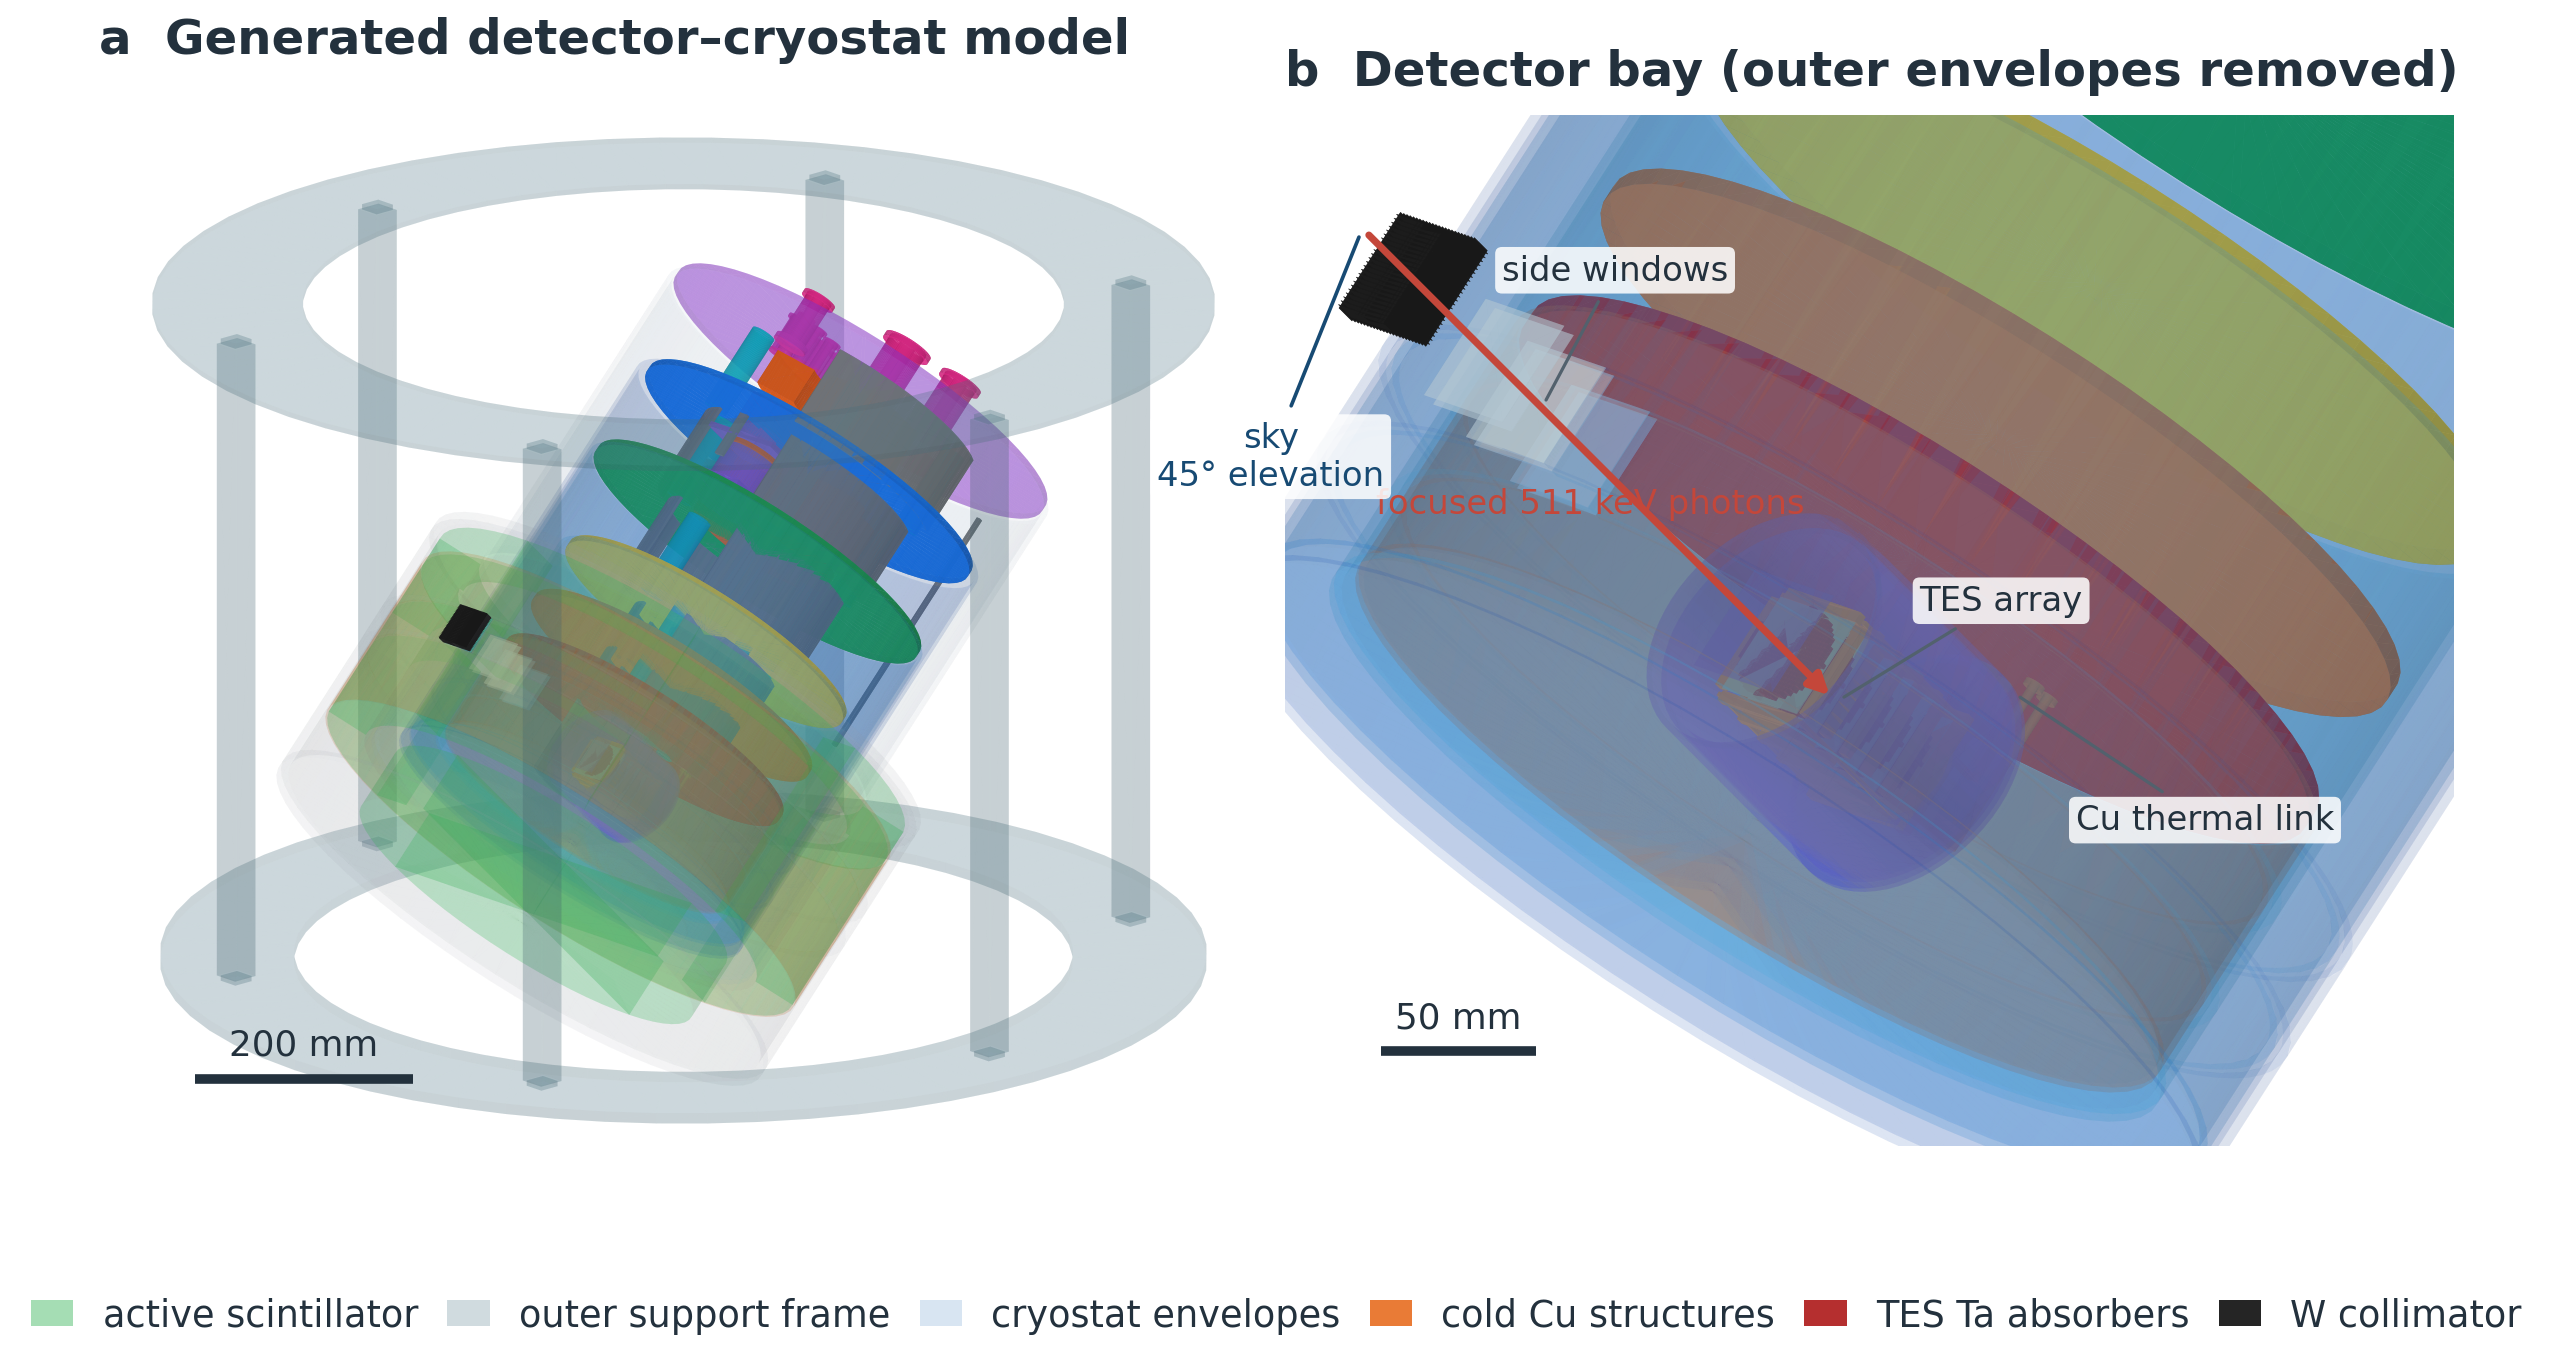
\includegraphics[width=0.98\linewidth]{paper_source_figure_table/fig_reference_detector_cryostat_geometry.png}
\caption{Schematic of the generic detector--cryostat mass-model template developed
during an earlier stage of this project. (a) Overview of the template, including the
outer support frame, active-scintillator shield, cryostat stages, and service
structures. (b) Detector-bay view with the outer envelopes hidden to show the TES
Ta array, copper thermal link, side-window stack, and W collimator. The aperture
axis is oriented at $45^\circ$ elevation; the red arrow indicates the nominal path
of focused 511 keV photons from the sky-facing collimator to the TES array.
Selected outer volumes are rendered translucent for clarity.}
\label{fig:mass_model}
\end{figure}

\FloatBarrier

\section{Simulation framework}
\label{sec:framework}

Detector-coupled Monte Carlo transport through detailed mass models was used to calculate the response and background of the 511\,keV spectrometer \cite{Sturner2003}. Figure~\ref{fig:workflow} summarizes the end-to-end calculation in three physical branches: focused signal, prompt atmospheric background, and delayed activation background. The Laue optics and the detector--cryostat system were represented by separate mass models. The reference point source was first transported through the Laue-lens model; the positions and directions of photons reaching the focal plane were written to a MEGAlib EventList and used to initialize detector-side Monte Carlo transport. For each design version, this focused-signal input and all background sources were transported through the same complete detector--cryostat mass model described in Section~\ref{sec:geometry}.

Broadband prompt transport and activation-production transport were run in parallel from the same EXPACS/PARMA atmospheric-field definition. The prompt branch contained two independently simulated inputs: the broadband gamma-ray continuum and particle fields supplied by EXPACS/PARMA, and a monoenergetic atmospheric positron-annihilation source at 511\,keV. The reference normalization of the latter was constrained by published atmospheric measurements \cite{Mahoney1981Atmospheric,Harris2003Atmospheric}. It was transported separately because the EXPACS/PARMA photon tables used here contain only continuum interpolation at 511\,keV, rather than a discrete line entry. In the delayed-activation branch, BUILDUP transport recorded nuclide yields, material volumes, and production positions. These records were used to calculate the activity accumulated during the flight and to construct the radionuclide inventory at the reference epoch; delayed decays were then sampled at the recorded production positions and transported through the detector--cryostat model.

The four detector-side event catalogues (focused signal, broadband prompt background, atmospheric 511\,keV line, and delayed activation) were processed with the same detector response, active-veto criterion, and Compton-topology test. The selected background events were decomposed by incident particle, parent nuclide, and production volume. This source decomposition was used to define and screen candidate shielding geometries. After the final candidate geometry had been fixed, its selected signal and component-resolved background rates were folded analytically over mission time and the adopted reference trajectory to obtain accumulated counts and unresolved-line sensitivity. Because a multi-day flight samples changing atmospheric and geomagnetic conditions, this fold does not simply scale a single Monte Carlo snapshot by elapsed time; its definitions and direct multi-point transport tests are given in Section~\ref{sec:mission_time_fold}. The terminal design-feedback node in Figure~\ref{fig:workflow} denotes the use of mission-scale assessment to constrain subsequent shielding refinement; it does not imply that the mission fold preceded definition and transport of the final candidate used in this study. The following subsections specify the source models, transport normalization, event-selection criteria, and trajectory calculation.

\begin{landscape}
\centering
\vspace*{\fill}
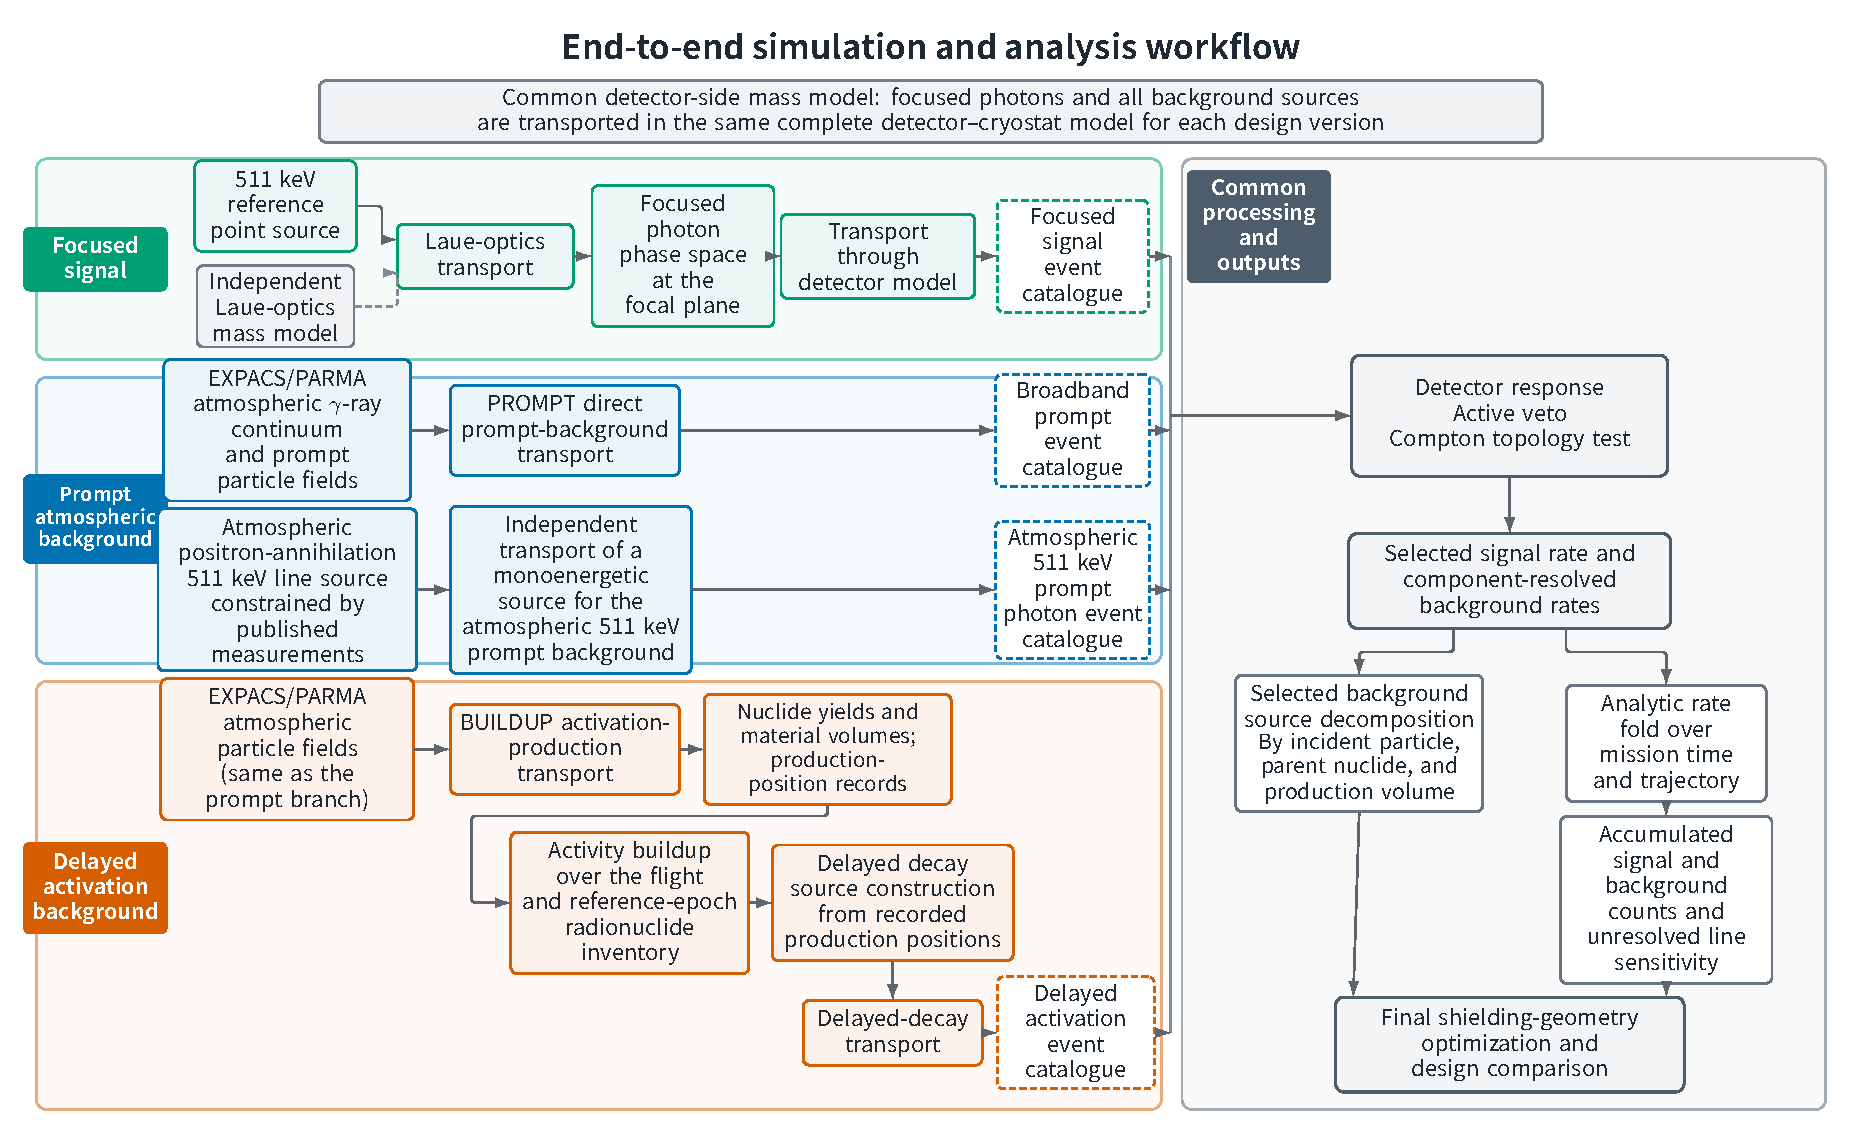
\includegraphics[width=0.94\linewidth]{paper_source_figure_table/fig_simulation_workflow_m04_en_20260810.pdf}
\captionof{figure}{End-to-end simulation and analysis workflow. Three physical branches produce four detector-side event catalogues: focused signal, broadband prompt background, the atmospheric 511\,keV prompt line, and delayed activation. All catalogues undergo the same detector response, active veto, and Compton-topology test. Background-source decomposition drives candidate-geometry screening; the reported mission fold is then evaluated for the fixed final candidate. The terminal node represents mission-scale feedback to subsequent design comparison and shielding refinement.}
\label{fig:workflow}
\vspace*{\fill}
\end{landscape}

\FloatBarrier

\subsection{Laue optics and detector-coupled signal transport}
\label{sec:optics}

This simulation adopts a laue-lens system based on mosaic Ge(111) crystals \cite{Barriere2009Laue,Barriere2011LauePrototype}. Through optical design, it realizes a 10 m focal length, a 511\keV{} single-ring reference response, and an effective area of $20.1\,\mathrm{cm^2}$ at 511\keV; the effective area is calculated as
\begin{equation}
  A_{\mathrm{eff}}(E)=A_{\mathrm{inc}}\frac{N_{\mathrm{fp}}(E)}{N_{\mathrm{inc}}(E)}
  \label{eq:laue_aeff}
\end{equation}
where $A_{\mathrm{inc}}$ is the Monte Carlo incident sampling area, $N_{\mathrm{inc}}(E)$ is the number of incident photons, and $N_{\mathrm{fp}}(E)$ is the number of photons satisfying the focusing/focal-plane interception condition.
The mosaic system is adopted to make the Monte Carlo calculation convenient while satisfying the expected focusing performance; other candidate schemes are also possible for actual engineering adaptation.

The Laue-optics branch calculates the focusing performance and explicitly transports the signal photons through the Ge crystal mass.

For this purpose, the diffraction probability of photons by the crystal is no longer superposed onto photons as an efficiency parameter, but is defined as a discrete process at the Geant4 application layer \cite{Agostinelli2003,Allison2016}. The process takes the diffraction probability $R(|\Delta\theta|)$ according to the angular deviation of the current photon relative to the crystal plane, and converts it into a finite equivalent diffraction mean free path $\lambda_{\mathrm{diff}}$, so that the accumulated diffraction probability when the photon crosses a crystal path $\ell$ reproduces this value: $1-\exp(-\ell/\lambda_{\mathrm{diff}})=R(|\Delta\theta|)$, namely $\lambda_{\mathrm{diff}}=-\,\ell/\ln[1-R(|\Delta\theta|)]$; to avoid double counting with standard photoelectric absorption, $R$ is first normalized by the unabsorbed fraction ($R/(1-A)$) and then converted into a mean free path. After this mean free path is returned to Geant4, the diffraction process and the standard electromagnetic processes (photoelectric absorption and Compton scattering) each sample interaction lengths in the same competition framework, and the shortest one decides which process occurs first, rather than forcibly intercepting photons at the crystal boundary. Photons not selected to undergo diffraction still continue transport according to the standard electromagnetic physics, and may be absorbed, scattered, or directly transmitted.

The diffraction probability is preferentially given by interpolation in an external XOP/CRYSTAL rocking-curve map as a function of angular deviation: this curve is calculated offline once in the preprocessing stage by the CRYSTAL/diff\_pat module of the XOP toolkit (called through xoppylib, with DABAX crystallographic data as input) \cite{SanchezDelRio2011XOP}, and gives the Ge(111) reflectivity/transmissivity/absorption curves as a function of angular deviation; during transport, the angular deviation is calculated in real time for every step inside the crystal, and the current diffraction probability is obtained by interpolation on that curve, namely ``offline library tabulation, probability used by angle during transport''. The mosaic orientation is implemented by applying a Gaussian angular perturbation to the ideal Bragg-plane normal, with the perturbation width given by the 30 arcsec mosaic FWHM; after diffraction occurs, the outgoing direction is mirror-reflected according to the perturbed plane normal, and the photon energy is unchanged. This split in which the ``process class only handles the transport interface, and the independent model class handles probability and direction decisions'' follows the idea of existing crystal Bragg-reflection extensions in Geant4 \cite{Guan2023BraggReflection,Reiazi2025G4BraggReflection}, and extends it to the energy band needed here.

Here the reference signal is a monochromatic 511\keV{} point source whose
rounded top-of-atmosphere flux scale
($\fzero=10^{-4}\phcms$, Section~\ref{sec:requirements}) is motivated by the
dedicated INTEGRAL/IBIS compact-source upper limit \cite{DeCesare2011}, rather
than by any single observed object. It is constructed as a MEGAlib far-field source
\cite{Zoglauer2006}, with the detailed construction given in
Section~\ref{subsec:pointsource}. The signal is transported through the optics
branch, and the recorded focal-plane crossing positions and directions are
converted into a MEGAlib EventList that seeds detector-side transport. Prompt
atmospheric backgrounds and activation decays are introduced independently in
the detector--cryostat model. The optics branch therefore supplies only the
focused-signal phase space, whereas the detector branch contains the signal and
all background streams used in the common response and selection analysis.

\subsection{Source construction}
\label{sec:background}

Within the three physical branches defined above, four detector-side inputs are
constructed independently: the focal-plane EventList for the reference point
source, the broadband prompt atmospheric field, the monoenergetic atmospheric
511\,keV line, and the delayed-decay source derived from the activation inventory.
The atmospheric line remains part of the prompt-background branch, whereas
activation production and delayed-decay transport remain separate stages. This
construction preserves the normalization and provenance of every input before the
common detector response and event selection are applied.

\subsubsection{Prompt atmospheric source}
\label{subsec:prompt_source}

The prompt atmospheric field is derived from EXPACS/PARMA. PARMA3.0 is an
analytical model parameterized from PHITS atmospheric-shower calculations and
benchmarked against terrestrial cosmic-ray measurements, and EXPACS is its
public tabulation and software interface
\cite{Sato2015EXPACS,Sato2016PARMA4}. PHITS supplies the underlying
particle-transport physics: primary cosmic rays interact with air nuclei, the
secondary hadrons, leptons, photons, and neutrons are transported through the
atmospheric column, and the resulting fluences are parameterized by altitude,
geomagnetic cutoff, solar modulation, energy, and direction. In this work
EXPACS/PARMA provides the differential incident flux as a function of particle
species, kinetic energy, zenith angle, geographic position, altitude, cutoff
rigidity, and solar activity, and is used only to construct the external
radiation fields; detector response, vetoing, topology selection, and
mission-time counting are applied downstream. The reference source definitions
use latitude $34^\circ$, longitude $100^\circ$, altitude $38\,\mathrm{km}$,
vertical cutoff rigidity $R_c=11.6\,\mathrm{GV}$, and the 2025-08-31 solar
condition corresponding to $W=118.3$.

The prompt source includes photons, neutrons, electrons, positrons, protons,
alpha particles, and negative and positive muons. For each particle family the
EXPACS/PARMA differential spectrum is converted into a MEGAlib far-field area
source covering the full zenith range $\theta=0^\circ$--$180^\circ$ and full
azimuth range $\phi=0^\circ$--$360^\circ$. The zenith dependence is represented
by 20 differential equal-$\mu$ angular bins, where $\mu=\cos\theta$ and each
bin subtends $\Delta\Omega=0.6283185307\,\mathrm{sr}$: the first ten bins cover
down-going particles, the last ten up-going or albedo-like particles. Both
hemispheres are retained in the prompt transport and in the
activation-production transport, so upward albedo particles are not discarded
at source construction. Figure~\ref{fig:expacs_fullsphere_flux} shows the
resulting full-sphere flux field.

\begin{figure}[t]
\centering
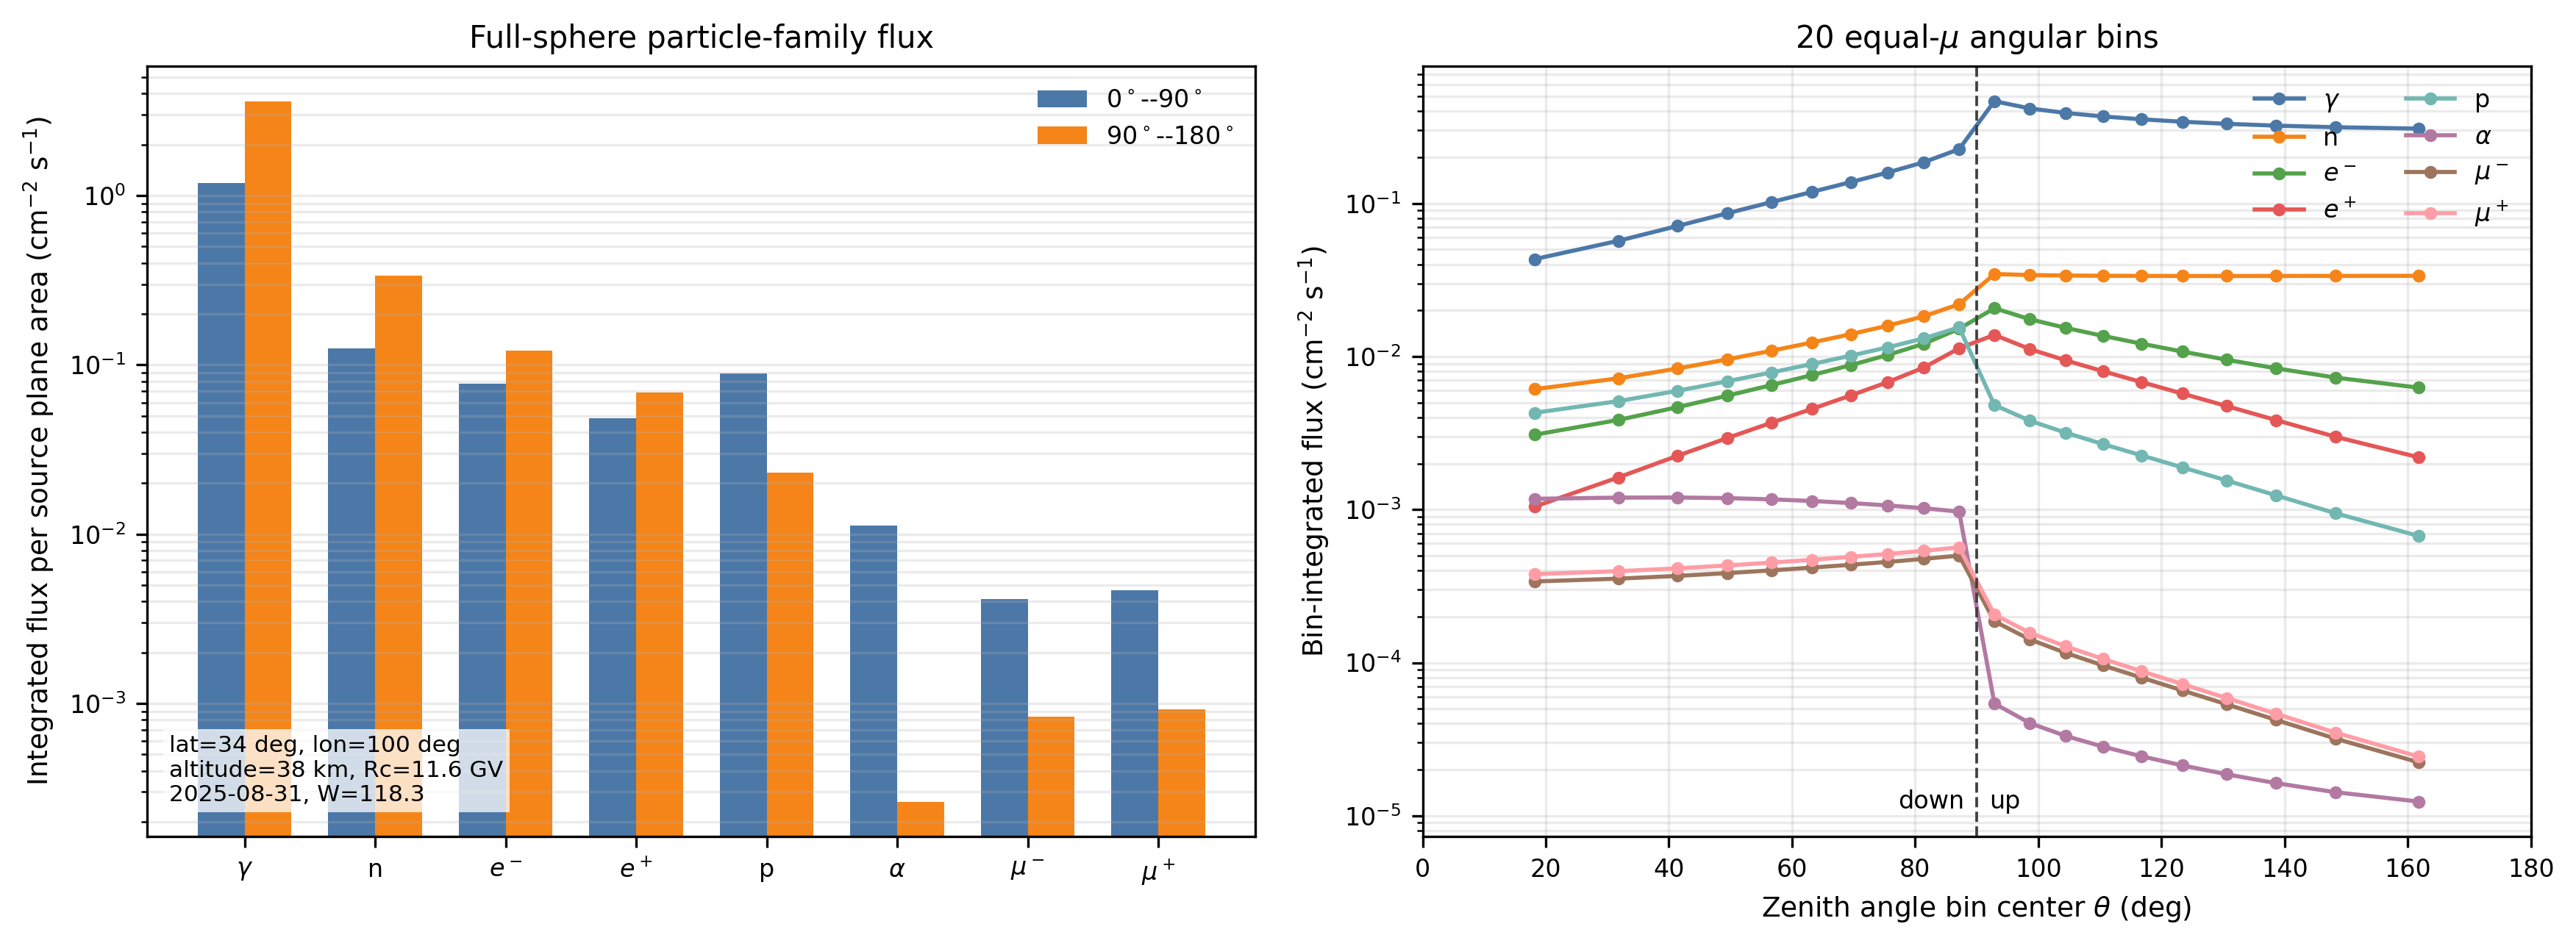
\includegraphics[width=\linewidth]{paper_source_figure_table/fig_expacs_fullsphere_flux.png}
\caption{EXPACS/PARMA full-sphere atmospheric flux field used to generate the prompt and activation-production transport inputs. Left: energy- and solid-angle-integrated fluxes for the eight transported particle families, separated into down-going and up-going hemispheres. Right: bin-integrated flux in the 20 equal-$\mu$ differential zenith bins used by the MEGAlib far-field source. The plot is generated from the source-definition inputs for latitude $34^\circ$, longitude $100^\circ$, altitude $38\,\mathrm{km}$, $R_c=11.6\,\mathrm{GV}$, and $W=118.3$.}
\label{fig:expacs_fullsphere_flux}
\end{figure}

The integrated source-plane fluxes are approximately $4.80$, $0.462$, $0.199$,
$0.117$, $0.112$, $0.0115$, $0.0050$, and $0.0056\,\mathrm{cm^{-2}\,s^{-1}}$
for $\gamma$, $n$, $e^-$, $e^+$, $p$, $\alpha$, $\mu^-$, and $\mu^+$,
respectively; the non-photon families together carry about
$0.91\,\mathrm{cm^{-2}\,s^{-1}}$, or 16\% of the total. If Monte Carlo counts
were allocated strictly in proportion to flux, the detector and activation
statistics of these minority families would be poor, so the non-photon
families are generated with replicated samples and de-weighted in the rate
normalization. All particles are then transported through the
detector/cryostat mass model with Geant4/MEGAlib
\cite{Agostinelli2003,Allison2016,Zoglauer2006}; the prompt run and the
activation-production run each generated 25,210,216 incident primaries. Each
particle species is normalized with its own transported exposure,
\begin{equation}
  r_{\mathrm{event},j}=\left(\sum_i \mathcal{T}_{ij}\right)^{-1},
\end{equation}
where $\mathcal{T}_{ij}$ is the transported exposure of subsample $i$ for
species $j$. This per-species normalization is required because the photon and
non-photon streams have different sampling and exposure structures; the
normalization check enforces $r_{\mathrm{event},j}\sum_i\mathcal{T}_{ij}=1$
for every species, so over-sampling changes the Monte Carlo variance but not
the expected physical rate.

\subsubsection{Atmospheric 511 keV line source}
\label{subsec:atm511_source}

The 20 atmospheric photon tables used for the EXPACS/PARMA prompt source represent
a smooth continuum. In every angular bin the tabulated energy grid has adjacent
entries at 449.65 and 566.08\,keV, so the value at 511\,keV is obtained by
continuum interpolation and not by an independent line entry. We retained these
tables unchanged and transported a separate atmospheric positron-annihilation
component modeled as monoenergetic at 511\,keV; detector broadening is applied in
the subsequent response stage. This numerical
separation does not establish that the smooth continuum is free of unresolved
annihilation-related emission. Possible overlap is therefore recognized as an
unquantified source-model uncertainty rather than assumed to be zero.

The line source is semi-empirical. Its reference normalization, rigidity factors,
and upward limb-darkening form are informed by atmospheric gamma-ray measurements
\cite{Mahoney1981Atmospheric,Harris2003Atmospheric}; the depth exponent,
hemispheric-ratio parameters, and downward angular kernel are modeling assumptions.
The full-sphere line-integrated flux is
\begin{equation}
  \Phi_{4\pi}(X,R_c)=\Phi_{\mathrm{ref}}\,f_R(R_c)
  \left(\frac{X}{X_{\mathrm{ref}}}\right)^{\eta} f_{\odot},
  \label{eq:atm511_flux}
\end{equation}
where the baseline uses $\Phi_{\mathrm{ref}}=0.10\,
\mathrm{ph\,cm^{-2}\,s^{-1}}$, $X_{\mathrm{ref}}=3.6\,
\mathrm{g\,cm^{-2}}$, $\eta=0.8$, and $f_{\odot}=1$. The adopted rigidity
factor is the step function
\begin{equation}
 f_R(R_c)=
 \begin{cases}
  1.000, & R_c<7\,\mathrm{GV},\\
  0.805, & 7\le R_c<9\,\mathrm{GV},\\
  0.624, & 9\le R_c<11\,\mathrm{GV},\\
  0.532, & 11\le R_c<13\,\mathrm{GV},\\
  0.479, & R_c\ge13\,\mathrm{GV}.
 \end{cases}
 \label{eq:atm511_rigidity}
\end{equation}
The downward-to-upward flux ratio and hemispheric fluxes are
\begin{equation}
  r_{\downarrow}(X)=\min\!\left[1,r_0
  \left(\frac{X}{X_{\mathrm{ref}}}\right)^{\beta}\right],\qquad
  \Phi_{\uparrow}=\frac{\Phi_{4\pi}}{1+r_{\downarrow}},\qquad
  \Phi_{\downarrow}=\frac{r_{\downarrow}\Phi_{4\pi}}{1+r_{\downarrow}},
  \label{eq:atm511_split}
\end{equation}
with $r_0=0.20$ and $\beta=0.5$.

Here $\theta$ is the source zenith angle: $\theta=0$ denotes photons arriving
from overhead and $\theta=\pi$ denotes upward/albedo photons. For the upward
hemisphere, $\mu_{\uparrow}=-\cos\theta$ and the normalized
limb-darkening law is
\begin{equation}
  I_{\uparrow}(\mu_{\uparrow})=
  \frac{\Phi_{\uparrow}}{2\pi(1+a/2)}(1+a\mu_{\uparrow}),
  \qquad a=1.7 .
  \label{eq:atm511_upward}
\end{equation}
For the downward hemisphere, $\mu_{\downarrow}=\cos\theta$ and the adopted
slab-production/escape kernel is
\begin{align}
  K_{\downarrow}(\mu_{\downarrow},X)
    &=1-\exp\!\left[-\frac{X}{\Lambda_{511}\mu_{\downarrow}}\right],
    &\Lambda_{511}&=11.5\,\mathrm{g\,cm^{-2}},\quad 0<\mu_{\downarrow}\le1, \notag\\
  I_{\downarrow}(\mu_{\downarrow},X)
    &=\frac{\Phi_{\downarrow}}{2\pi\mathcal{A}(X)}
      K_{\downarrow}(\mu_{\downarrow},X),
    &\mathcal{A}(X)&=\int_0^1K_{\downarrow}(\mu,X)\,\mathrm{d}\mu .
  \label{eq:atm511_downward}
\end{align}
The continuous limit $K_{\downarrow}(0,X)=1$ is used at the horizon. The
attenuation scale is consistent with the dry-air mass attenuation coefficient
near 511\,keV \cite{NISTXCOM}.

The full sphere is discretized into the same 20 equal-$\mu$ bins used by the
prompt source, with 10 bins in each hemisphere, $\Delta\mu=0.1$, and
$\Delta\Omega=2\pi\Delta\mu=0.628319\,\mathrm{sr}$. MEGAlib
samples the far-field area sources on the projected disk
associated with a 60\,cm start sphere centered at $(5,0,9)$\,cm; the normalization
uses $A_{\mathrm{proj}}=\pi R^2=1.13097\times10^4\,\mathrm{cm^2}$ rather than
the physical surface area $4\pi R^2$. At the day-15 proxy state used by the
line-transport source card, $X=3.46147\,\mathrm{g\,cm^{-2}}$ and
$R_{c,\mathrm{line}}=11.0\,\mathrm{GV}$ give $\Phi_{4\pi}=0.0515559\,
\mathrm{ph\,cm^{-2}\,s^{-1}}$, with $\Phi_{\uparrow}=0.0431028$ and
$\Phi_{\downarrow}=0.00845307\,\mathrm{ph\,cm^{-2}\,s^{-1}}$. The Monte Carlo
transport generated $3.0\times10^6$ photons, corresponding to an effective
exposure of 5143.83\,s and a per-event rate weight of
$1.94408\times10^{-4}\,\mathrm{s^{-1}}$. The state-specific PARMA field used
for prompt and activation scaling has $R_{c,\mathrm{PARMA}}=11.6\,\mathrm{GV}$
at day 15. Both values lie in $11\le R_c<13\,\mathrm{GV}$ and therefore use the
same $f_R=0.532$; the atmospheric-line branch retains its separate proxy rigidity
curve in the mission fold.

\subsubsection{Delayed activation source}
\label{subsec:delayed_source}

For the delayed simulation, a separate activation-production stream is run by
enabling BUILDUP during the prompt-background transport. This
activation-production stream is not counted as an immediate detector background.
Instead, it records the isotope, material volume, and production position of
each radioactive product. These records are converted through the
production--decay accumulation equation into a radioactive population fixed to a
chosen reference time during the flight, with ground-state half-lives checked
against NUBASE2020 \cite{Kondev2021NUBASE}. For isotope $k$,
\begin{equation}
  A_k(t_{\mathrm{flight}}) = P_k\left[1-\exp\left(-\lambda_k t_{\mathrm{flight}}\right)\right],
  \qquad \lambda_k = \frac{\ln 2}{t_{1/2,k}},
\end{equation}
where $P_k$ is the production rate inferred from the activation-production
transport and $t_{\mathrm{flight}}=15\,\mathrm{d}$ for the reference state.
The fixed delayed total activity used by the mass-complete reference
delayed-source construction is $141.83\,\mathrm{Bq}$. This reference value is
retained for the background-origin comparison below; the final directionally graded chain has
its own all-eight-family inventory and normalization.

The position information does not come from the aggregate isotope store alone.
The standard store records volume names and isotope counts; the
production-position construction adds a custom recording hook in the MEGAlib
stepping-action layer. Whenever a delayed isotope is stored during activation
buildup, the hook writes a production-position record at the same moment,
including the logical volume name, pre-step position $(x,y,z)$, isotope
identifier $1000Z+A$, excitation energy, time, process, and track-ancestry
information. The fixed day-15 population is then matched to these records by
volume, isotope, and excitation state, so the delayed source can use the
simulated production coordinates rather than only volume-integrated activities.
The reference-detector inventory is summarized by production volume, nuclide,
incident family, material category, and production coordinate. These are
source-construction quantities rather than detector counts; detector response is
applied only after the delayed decays are transported through the common geometry
and event selection.

Whether the production positions are worth preserving can be tested from the
same table. Delayed decays are emitted locally, so downstream attenuation,
active-shield veto probability, and event topology all depend on where the
isotope was produced, and different incident families---with their different
energy-loss, stopping, and capture histories---need not deposit their
activation in the same materials. To quantify this, the weighted production
rows are grouped by incident particle family and material category, and the
activity-normalized category distributions of two families $a$ and $b$ are
compared with the total-variation distance
\begin{equation}
  D_{\mathrm{TV}}(a,b) =
  \frac{1}{2}\sum_c \left| f_{a,c} - f_{b,c} \right| ,
\end{equation}
where $f_{a,c}$ is the fraction of delayed activity from family $a$ produced
in material category $c$. Production volumes are grouped as active CsI,
outer mechanical structures, cold plates, passive tungsten/collimator material,
window material, TES volumes, and other internal structures. A volume-integrated
or axisymmetric radial source could preserve the total
activity, but it would erase these incident-family, material, nuclide, and
coordinate correlations; the production-position construction keeps them in
the source before detector transport.

The delayed-decay source is therefore emitted from sampled production positions
rather than from an axisymmetric distribution. Let row $j$ in the weighted
production table have activity weight $w_j$, with total activity
$A=\sum_j w_j$. During construction, $M$ production positions are drawn with
replacement using probability $p_j=w_j/A$, and each sampled point source is
assigned the same flux $A/M$. The expected activity assigned to row $j$ is
\begin{equation}
  \mathbb{E}\!\left[N_j\frac{A}{M}\right] = M p_j \frac{A}{M} = w_j ,
\end{equation}
so the estimator preserves the total activity and is unbiased for the weighted
spatial distribution. Here $M$ is the number of equal-activity sampled point
sources; it is a sampling size, not the number of physical production rows. The
reference delayed source preserves the fixed total activity at the
source-definition level and is transported through the same detector/cryostat
geometry as the prompt stream. The nominal calculation transports $10^6$
delayed decays; the corresponding Cosima live time is only the transport record
used to generate the decay sequence and is not used as the physical balloon
exposure time.

Table~\ref{tab:background_source_model} summarizes the source layers used in the
current detector-coupled calculation. It is placed in the source-model section
because this section defines incident particle fields and delayed radioactive
populations; detector vetoes and topology selections are applied only in the
subsequent selection section.

\begin{table}[t]
\centering
\caption{Background-source layers used by the current detector-coupled chain. The table defines source construction only; anticoincidence, topology selection, and the line window are applied later in Section~\ref{sec:selection}.}
\label{tab:background_source_model}
\begin{tabular}{p{0.22\linewidth}p{0.34\linewidth}p{0.34\linewidth}}
\hline
Layer & Physical role & Current implementation \\
\hline
Prompt atmospheric transport & Direct detector hits from atmospheric secondaries & EXPACS/PARMA full-sphere source definitions at $34^\circ$ latitude, $100^\circ$ longitude, $38\,\mathrm{km}$ altitude, $R_c=11.6\,\mathrm{GV}$, and $W=118.3$; $\gamma$, $n$, $e^\pm$, $p$, $\alpha$, and $\mu^\pm$ over 20 equal-$\mu$ differential zenith bins including both down-going and up-going hemispheres; 25,210,216 generated primaries. \\
Atmospheric 511\,keV line & Atmospheric positron-annihilation photons that are spectrally degenerate with the science line & Separate monoenergetic full-sphere component over 20 equal-$\mu$ bins (10 per hemisphere); day-15 $\Phi_{4\pi}=0.0515559\,\mathrm{ph\,cm^{-2}\,s^{-1}}$; $3.0\times10^6$ generated photons, 5143.83\,s effective exposure. \\
Activation production & Radioisotope production and production-position history & Same atmospheric field transported as a BUILDUP activation-production stream, again retaining both hemispheres and all eight particle families; 25,210,216 generated primaries. \\
Fixed delayed population & Radioactive activity at the adopted day-15 state after continuous exposure & Production--decay accumulation with NUBASE-checked ground-state half-lives; $141.83\,\mathrm{Bq}$ for the mass-complete reference and $36.4525153\,\mathrm{Bq}$ for the final directionally graded configuration. \\
Production-position decay transport & Delayed decay particles emitted from sampled production positions & Equal-activity sampled point sources from the weighted production table; the final configuration transports $10^6$ delayed triggers for each of seven positive activation families, while the electron-minus family is a finite-buildup zero observation with no fictitious transport exposure. \\
\hline
\end{tabular}
\end{table}

This production-position representation does not create one sampled point source
for every production row. Each positive-family realization uses $M=50{,}000$
sampled positions and transports $10^6$ delayed triggers. We first verify activity
conservation and source serialization, then propagate the same realization
through the detector response and event selection. The resulting selected rate
and its nuclide/volume decomposition are reported in
Section~\ref{subsec:reference_background_results}.

The $141.83\,\mathrm{Bq}$ all-family day-15 inventory above is used to identify
the activation origins of the mass-complete reference geometry, whose 26 selected
delayed records remain 24 $^{64}$Cu and two $^{61}$Cu records. The final
graded-shield calculation instead uses the NUBASE-corrected all-eight-family
inventory of $36.4525153\,\mathrm{Bq}$ at day 15. The seven positive activation
families with delayed transports are $\alpha$, $e^+$, $\gamma$, $\mu^-$, $\mu^+$,
$n$, and $p$; the finite BUILDUP sample for $e^-$ observed no production, so its
central delayed contribution is zero and no transport exposure or Garwood bound
is invented. The primary response realization retains 78 delayed records after
the complete detector selection (1 $\alpha$, 5 $\mu^-$, 60 $n$, and 12 $p$;
the other positive transported families retain zero final records).

The finite $M$ sampling is an additional source-level boundary rather than a
Poisson counting interval. In the dominant neutron realization, undrawn
low-probability nuclide--volume species carry $0.157388\,\mathrm{Bq}$, or
$0.515\%$ of the neutron activity. This missed sampled-species fraction is
reported explicitly and is not covered by the componentwise Garwood endpoint.
One retained neutron event also begins in the SIM record as the daughter
$^{182}$W; its production position uniquely maps it back to the radioactive
source parent $^{182}$Ta. Mission-time activity and response are therefore keyed
to the $^{182}$Ta parent, while the $^{182}$W IA INIT identity is retained as
transport-lineage evidence.

\subsubsection{Reference point-source construction}
\label{subsec:pointsource}

The focused signal stream is defined by a monochromatic 511\keV{} reference
point source. Its flux scale is set not by any single observed object but by a
rounded comparison to the dedicated INTEGRAL/IBIS compact-source limit:
$\fzero=10^{-4}\phcms$ at the top of the atmosphere
(Section~\ref{sec:requirements}) \cite{DeCesare2011}.

Because such a source lies at astronomical distance, it is modelled as an ideal
on-axis point: in the optics run it is a monochromatic 511\keV{} far-field beam
whose photons arrive parallel to the optical axis and are sampled uniformly over
the incident aperture $A_{\mathrm{inc}}$ of Eq.~(\ref{eq:laue_aeff}). No finite
angular size is assigned to the source itself; the angular structure that reaches
the focal plane is produced entirely by the lens---the 30 arcsec mosaic spread,
the XOP/CRYSTAL rocking curve, and the $f=10\,\mathrm{m}$ focusing geometry---so
that the photons recorded at the focal plane converge to within about $0.4^\circ$ of the axis and
forms a focused spot rather than a single ray. Three independent seeds of
$5\times10^{4}$ primaries each give $1.5\times10^{5}$ transported photons, of
which 37,256 are diffracted and cross the focal plane; 37,194 of these (99.8\%)
fall within the $r=1.898\,\mathrm{cm}$ Be entrance window, with focused-spot
radii $r_{90}=1.03\,\mathrm{cm}$ and $r_{99}=1.25\,\mathrm{cm}$. The
within-window crossings form a MEGAlib EventList source. Each entry supplies
its recorded position and direction at the Be aperture and initiates a new
detector-side Monte Carlo transport through the detector/cryostat model.

The EventList-source normalization relates the detector-side transport to the reference flux. At the detector
entrance the focused stream carries the rate
\begin{equation}
  R_{\mathrm{fp}}=F_{\mathrm{TOA}}\,\aeff(511\keV)\,T_{\mathrm{atm},45} .
\end{equation}
Here
$\aeff(511\keV)=20.1\,\mathrm{cm^2}$ is the on-axis Laue effective area,
$F_{\mathrm{TOA}}$ is defined at the top of the atmosphere, and
$T_{\mathrm{atm},45}=0.6520$ is the day-15 transmission along the fixed
$45^\circ$-elevation axis; numerically this is $1.31\times10^{-3}\cps$ at the
reference flux.
Equivalently, the generating run corresponds to an observation time
$N_{\mathrm{fp}}/[F_{\mathrm{TOA}}\,\aeff\,T_{\mathrm{atm},45}]$, and each EventList entry carries the inverse
of that exposure as its rate weight; in the intermediate cut-flow bookkeeping of
Section~\ref{sec:selection} the same sample is initially normalized to a unit EventList input rate before this
scale is applied. After the common detector response and event selection, the
surviving signal rate is $9.86228\times10^{-4}\cps$. Dividing out the atmosphere
gives an instrument-only selected effective area
$A_{\mathrm{sel,instr}}=S_{\wii}/(\fzero T_{\mathrm{atm},45})=15.1254\,\mathrm{cm^2}$;
the atmosphere-folded conversion from top-of-atmosphere flux to selected rate is
$S_{\wii}/\fzero=9.8623\,\mathrm{cm^2}$. Because the optics run
contains only source photons, the EventList source contains only signal photons; all
backgrounds enter through the streams of Section~\ref{sec:background}.

The effective area quoted above is the on-axis value, representing best-case
pointing. A point source offset from the optical axis, or residual attitude
jitter during flight, reduces and shifts the focused response through the finite
angular acceptance (field of view) of the Laue lens
\cite{Barriere2009Laue,Weidenspointner2006MAX}; this off-axis dependence is
treated as a pointing systematic on the signal effective area rather than as a
change to the on-axis reference construction. The current side-entry response
is a fixed $45^\circ$-elevation reference, not a simulated
low-elevation Galactic-centre observation.

\subsection{Background-led geometry design and statistical treatment}
\label{subsec:comparison_hierarchy}

The geometry design begins with the background that reaches the science window.
For the mass-complete reference calculation, we group final events by incident
particle family and, for delayed events, by parent isotope and production volume.
The prompt map identifies the directions that require active coverage; the delayed
map identifies nearby materials that feed the line window after activation. This is
the same component-first logic used in detailed COSI and DIXE background studies
\cite{Gallego2025Balloon,Tian2026DIXE}. It leads to the final graded-shield geometry used for
the full calculation: 40 mm BGO around the side, a 30 mm bottom disk, and a 10 mm
top annulus. The side optical aperture, 3 mm Al mechanical shell, Kapton layer,
detector, and cryostat are retained, and there is no external W layer. The final
geometry is thus described by one physical question: where is active coverage most
useful for the line-window background?

Before these stages, Cosima energy deposits are aggregated by TES pixel. Each
pixel readout then receives an independent Gaussian energy response with
$\Delta E_{\mathrm{FWHM}}=0.420\keV$ ($\sigma=0.17836\keV$); measured hits below
$0.3\keV$ are discarded, and the surviving measured hits are summed before the
line window, active veto, and topology tests. The focused, prompt, and delayed
catalogues use fixed response seed 26071301, while the independently convolved
atmospheric-line catalogue uses fixed seed 1026071308. With Gaussian broadening disabled, the response
calculation reproduces the transport-level cut-flow exactly. A 64-realization
response ensemble assesses numerical stability and is used as a numerical
response-integration check rather than as an additional physical systematic.

All signal and background streams are summarized at three common stages: after the
energy window, after the active veto, and after the topology/field-of-view test. For
stream $k$ and stage $j$, the physical rate and its Monte Carlo counting error are
\begin{equation}
  \widehat R_{k,j}=\sum_{i\in(k,j)} w_i,
  \qquad
  \sigma_{k,j}=\left(\sum_{i\in(k,j)} w_i^2\right)^{1/2},
  \qquad
  N_{\mathrm{eff},k,j}=\frac{\widehat R_{k,j}^{2}}{\sigma_{k,j}^{2}},
  \label{eq:weighted_rate_stats}
\end{equation}
where $w_i$ is the physical rate carried by record $i$. We also report the stage
survival $q_{k,j}=\widehat R_{k,j}/\widehat R_{k,\mathrm{window}}$ and the final
background share $f_k=\widehat R_{k,\mathrm{final}}/\sum_b
\widehat R_{b,\mathrm{final}}$. Counts and rates are both shown because the streams
have different exposure weights: counts measure Monte Carlo support, whereas rates
measure the physical background.

Within an independently normalized transported component the event weights are
constant, so a two-sided 95\% Garwood interval for the Poisson count can be
multiplied by the component weight to obtain an exact rate interval. A zero
selected count with a defined transport exposure is treated in the same way and
therefore gives an upper limit rather than a zero-background claim. The finite-
BUILDUP $e^-$ family is different: no delayed source or transport exposure exists,
so no fictitious Garwood limit is assigned. Focused-signal acceptance is binomial;
its two-sided 95\% interval is Clopper--Pearson. The central mission projection
uses the estimated rates. A second, conditional componentwise transport-counting
endpoint uses the upper Garwood endpoint for every transported background
component and the lower Clopper--Pearson endpoint for the signal. Summing these
component endpoints is not a joint-coverage interval and is not full 95-percent
coverage; it excludes BUILDUP-yield, finite-$M$ position sampling,
zero-family, nuclide-mixture, radiation-field, cross-section, and detector
systematics. These calculations used SciPy~1.8.0.

For time bin $\ell$, live fraction $L_\ell$, and duration $\Delta t_\ell$, the
cumulative signal and background counts are
\begin{equation}
 N_s(T)=\sum_{\ell\leq T} S_\ell L_\ell\Delta t_\ell,
 \qquad
 N_b(T)=\sum_{\ell\leq T} B_\ell L_\ell\Delta t_\ell.
 \label{eq:cumulative_counts}
\end{equation}
We use the transparent counting metric $Z(T)=N_s(T)/\sqrt{N_b(T)}$. Because the
signal rate is linear in source flux, the corresponding diagnostic threshold is
$F_{3\sigma}(T)=F_0\,3/Z(T)$. The central curve and the conditional componentwise
transport-counting endpoint are propagated through the same 81-bin trajectory.
Their separation measures finite transported Monte Carlo support under the stated
conditioning; it is not a confidence band for atmospheric fields, cross sections,
or detector calibration.

\subsection{Detector event selection and veto definitions}
\label{sec:selection}

The reference coincidence calculation places the focused-signal, prompt
atmospheric, and delayed-activation catalogues on one explicit time axis and
applies two veto layers in sequence. The independently transported atmospheric
511\,keV catalogue receives the same detector response and event-wise selection.
Its full-band detector occupancy is added to the final mission-time live-factor
calculation, as specified below. This distinction separates the reference
three-catalogue coincidence demonstration from the final four-component rate
budget.

\subsubsection{Time axis and rate normalization}

Each stream enters with a per-record rate weight $r_{km}$ from the source
normalization of Section~\ref{sec:background}, where $k$ labels the stream and
$m$ labels a record in that stream's event catalogue; the stream total rate is
$R_k=\sum_m r_{km}$. To place three independently normalized catalogues on one
physical time axis, the streams are combined by a Poisson superposition: for
stream $k$ the number of instances is drawn as
\begin{equation}
  N_k\sim \mathrm{Pois}(R_k T),
\end{equation}
records are selected with probabilities $r_{km}/R_k$ with replacement, each is
assigned a uniform random time in the reference window $[0,T]$, and all streams
are merged and time-ordered into a single detector time axis carrying the three
physical rates. Event instances separated by no more than $\tau=1\,\mu\mathrm{s}$
are grouped into a coincidence candidate group $c$. In the reference validation (Figure~\ref{fig:s33_poisson}) the full-band detector rates superposed on this axis are about $928\,\mathrm{s^{-1}}$ (prompt), $97.1\,\mathrm{s^{-1}}$ (delayed activation), and $0.987\,\mathrm{s^{-1}}$ (focused signal), so the coincidence axis is strongly prompt-dominated; over the reference exposure the $7{,}215{,}233$ event instances yield 1275 mixed-stream coincidences, giving an accidental live factor $\simeq0.9990$ (the line window and shield threshold below then act on the resulting candidate groups). The normalized summed-energy spectrum of these three reference streams is shown in Figure~\ref{fig:s33_spec_norm}: the window is line-dominated, with a sparsely sampled continuum.

\begin{figure}[t]
\centering
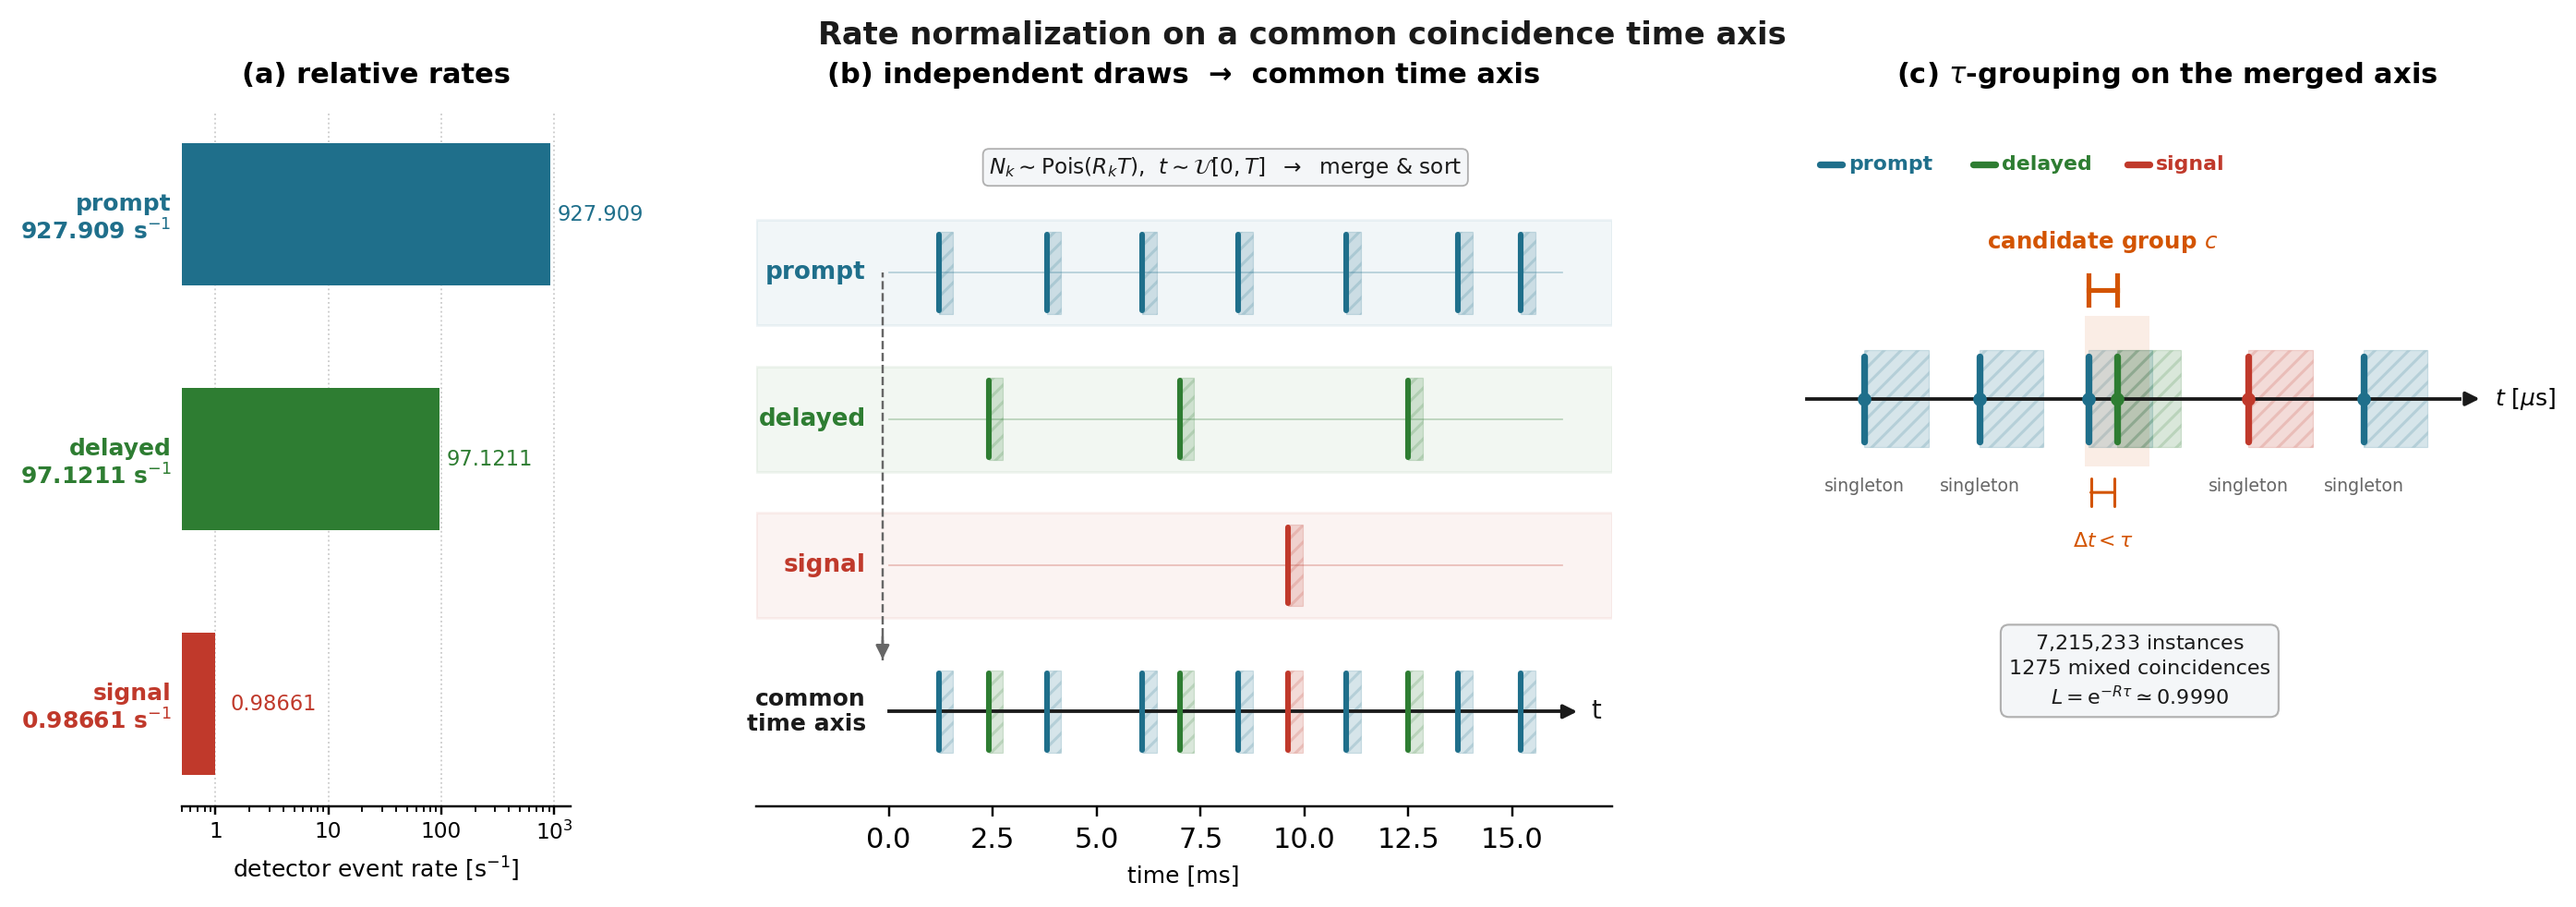
\includegraphics[width=\linewidth]{paper_source_figure_table/fig_s33_poisson_normalization.png}
\caption{Reference three-stream validation of rate normalization on a common coincidence time axis. (a)~Full-band detector event rates ($928$, $97.1$, and $0.987\,\mathrm{s^{-1}}$). (b)~Independent Poisson draws of the three streams are merged and time-ordered; color marks stream identity and hatched bands mark each event's temporal footprint. (c)~Events with $\Delta t\le\tau=1\,\mu\mathrm{s}$ form one candidate group; the box gives the reference-exposure accidental-coincidence accounting. Tick positions are schematic. The final mission fold additionally includes atmospheric-line occupancy through Equation~\eqref{eq:atm511_live_factor}.}
\label{fig:s33_poisson}
\end{figure}

\begin{figure}[t]
\centering
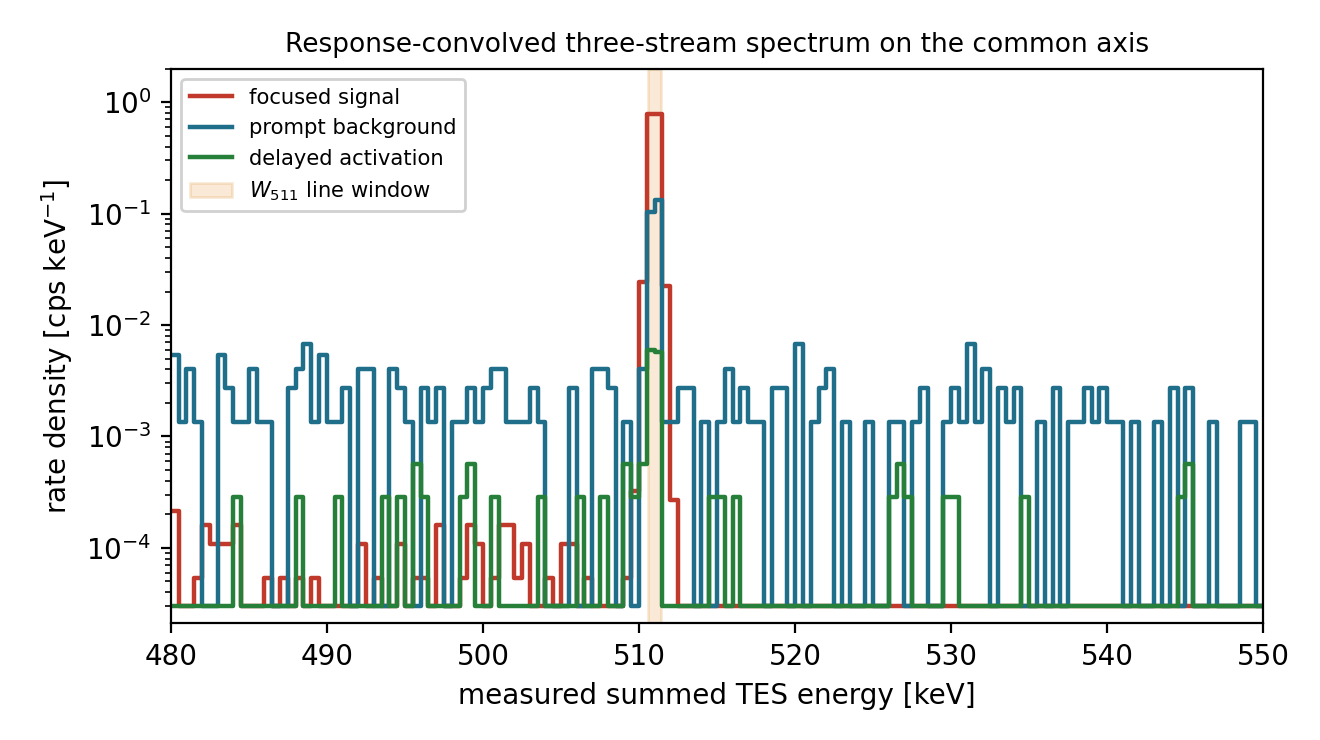
\includegraphics[width=0.72\linewidth]{paper_source_figure_table/fig_s33_spectrum_normalized.png}
\caption{Response-convolved summed-energy spectra of the three reference streams on the
common axis before vetoes. The focused signal, prompt, and delayed streams all
concentrate at the 511\keV{} line while the continuum is sparsely sampled. Absolute
selected line-window rates are given in Table~\ref{tab:phase2_cutflow}.}
\label{fig:s33_spec_norm}
\end{figure}

The explicit Poisson realization in Figures~\ref{fig:s33_poisson} and
\ref{fig:s33_spec_norm} is a reference validation and does not contain the
atmospheric-line catalogue. In the final trajectory calculation, the selected
atmospheric-line rate is propagated separately and its detector occupancy is
included in the live fraction for time bin $\ell$:
\begin{equation}
  L_{\ell}=\exp\!\left\{-\tau\left[
  R^{\mathrm{occ}}_{\mathrm{prompt},\ell}+
  R^{\mathrm{occ}}_{\mathrm{delayed},\ell}+
  R^{\mathrm{occ}}_{\mathrm{atm511},\ell}\right]\right\}.
  \label{eq:atm511_live_factor}
\end{equation}
At the line-source day-15 reference, the atmospheric catalogue contains
$1{,}041{,}505$ events with at least one TES or active-shield hit, giving
$R^{\mathrm{occ}}_{\mathrm{atm511}}(15)=202.477\,\mathrm{s^{-1}}$. The focused
full-band rate at the reference source flux is $0.987\,\mathrm{s^{-1}}$, so
$R^{\mathrm{occ}}_{\mathrm{sig}}\tau\simeq9.9\times10^{-7}$ and signal
self-coincidence is neglected under the weak-source approximation. A brighter-source
application would require adding $R^{\mathrm{occ}}_{\mathrm{sig},\ell}$ to the
exponent.
The active anticoincidence gate compares TES and active-shield deposits within
the same $\tau$ window, and the topology reconstruction determines which hits
belong to one incident photon. The same coincidence window and shield threshold
are used for every transported component. Within each trajectory bin the rates
are treated as stationary: the atmospheric column and activation inventory evolve
on mission-day scales, whereas the coincidence calculation spans microseconds to
seconds. Independent constant-rate arrivals may therefore be superposed as
homogeneous Poisson processes. The mission fold uses their expectation values
rather than adding a new stochastic realization in every bin; the explicit
three-stream realization validates only the grouping and accidental-coincidence
accounting.

\subsubsection{Active anticoincidence gate}

The first layer is an active anticoincidence gate on this common time axis. For
each candidate group $c$ the TES and active-shield energy sums are
\begin{equation}
  E_{\mathrm{TES}}^{(c)}=\sum_{j\in c}E_{\mathrm{TES},j},\qquad
  E_{\mathrm{sh}}^{(c)}=\sum_{j\in c}E_{\mathrm{sh},j}.
\end{equation}
The group enters the hard line window if $E_{\mathrm{TES}}^{(c)}$ falls in
\begin{equation}
  \wii = [510.58,511.42]\keV \quad (511\keV\pm420\,\mathrm{eV}),
\end{equation}
which is the primary reference selection window, retaining most of the line response while
suppressing continuum background. The group passes the active shield if
\begin{equation}
  E_{\mathrm{sh}}^{(c)} < E_{\mathrm{veto}}, \qquad E_{\mathrm{veto}}=50\keV,
\end{equation}
where for the baseline CsI configuration the shield sum is read from the CsI
active-shield volumes in post-processing. This layer is the dominant source of
rate-level background suppression. After the per-pixel detector response and
threshold are applied, it reduces the prompt background from 148 to 68 events
($0.1146\to0.04612\cps$, $40.24\%$ surviving) and delayed activation from 40
to 26 events ($65.00\%$), while retaining all 28534 focused-signal events
(zero shield deposit, $100\%$); see Table~\ref{tab:phase2_cutflow}. Its effect
on the background spectrum is shown in Figure~\ref{fig:s33_spec_anti}.

\begin{figure}[t]
\centering
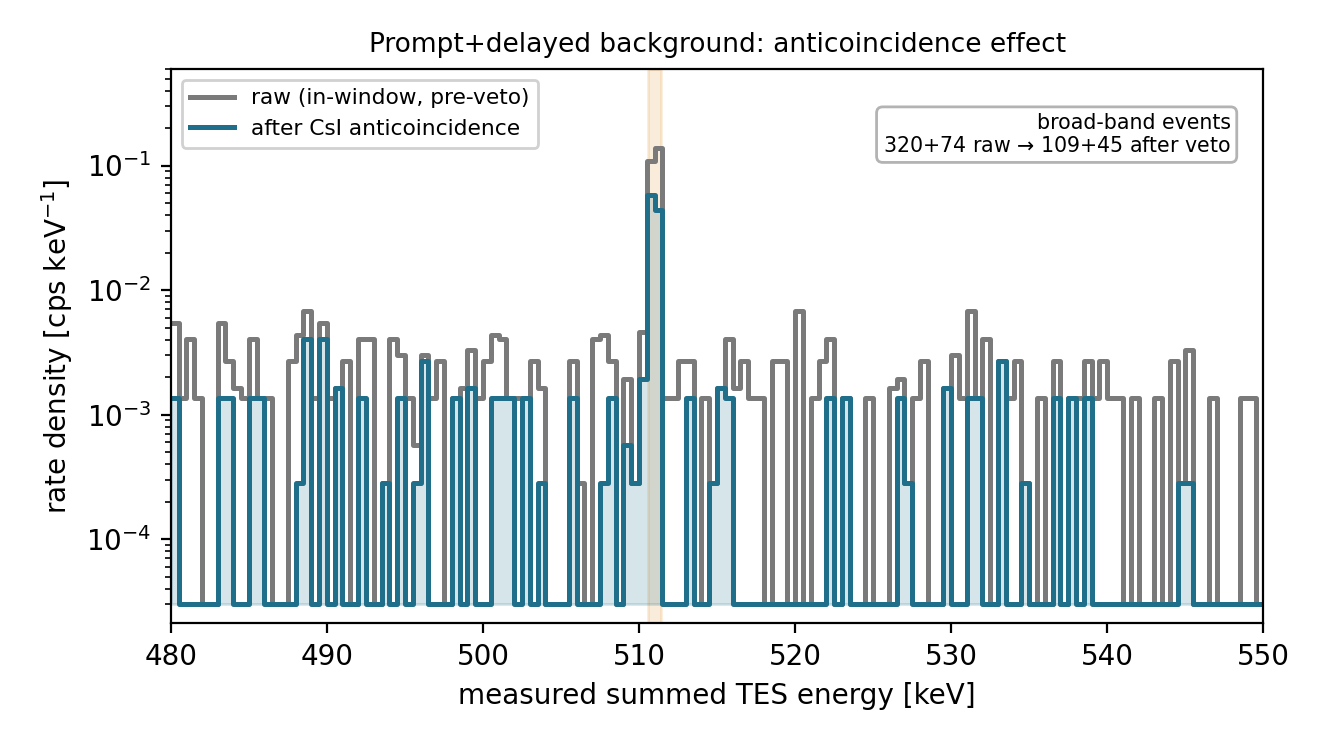
\includegraphics[width=0.72\linewidth]{paper_source_figure_table/fig_s33_spectrum_anticoincidence.png}
\caption{Effect of the CsI anticoincidence gate on the prompt$+$delayed background spectrum (in-window pre-veto vs after the shield gate). Shape-diagnostic re-derivation on the surviving reference-detector catalogues.}
\label{fig:s33_spec_anti}
\end{figure} The quoted flux thresholds apply to a line
whose intrinsic width, after detector response, remains small compared with this
window; a substantially broadened source line would require convolving the
source line profile with the response and re-optimizing the window.

\subsubsection{Compton topology and field-of-view consistency}

The second layer applies a Compton-kinematic topology and field-of-view
consistency test to the TES hits that survive the active-shield gate; its
physical basis is Compton-camera cone reconstruction \cite{Zoglauer2006}. An
incident photon of energy $E_0$ Compton-scatters at a first interaction point
$\mathbf r_1$, depositing $E_1$, and the scattered photon of energy
$E_{\mathrm{sc}}=E_0-E_1$ propagates to a second interaction point $\mathbf r_2$;
the scattering angle follows from
\begin{equation}
  \cos\theta_C =
  1 - m_ec^2\left(\frac{1}{E_{\mathrm{sc}}}
  - \frac{1}{E_1+E_{\mathrm{sc}}}\right).
\end{equation}
Given the scattered-photon direction
$\hat{\mathbf u}_{12}=(\mathbf r_2-\mathbf r_1)/|\mathbf r_2-\mathbf r_1|$, the
source direction is constrained to a reconstruction cone with apex $\mathbf r_1$,
axis $-\hat{\mathbf u}_{12}$, and half-angle $\theta_C$, whose projection on the
sky is the event circle. We use this first-scatter cone as an aperture-consistency
test: the event is retained when the cone intersects the side Be-window disk (radius
$1.898\,\mathrm{cm}$), i.e.\ whether the reconstructed arrival direction is
consistent with entry through the aperture.

Because the interaction position within a single TES pixel
($1.5\times1.5\times3.0\,\mathrm{mm}$) is unresolved, each hit is represented not
by its centroid alone but by $8+1=9$ representative points---the eight pixel
corners and the centroid---carrying the sub-pixel position uncertainty
explicitly into the geometric reconstruction. A two-hit event in a given scatter
order therefore enumerates $9\times9=81$ first/second position combinations and
constructs one reconstruction cone per combination (each cone sampled at 24
azimuths, propagated to the Be-window plane, and tested against the disk by both
its sampled points and the connecting segments); the order is deemed
field-of-view consistent if any of these 81 trajectories yields a cone that
intersects the disk. This is a deliberately permissive consistency test: an
event is retained if any sub-pixel interaction position is consistent with entry
through the aperture. The layer consequently retains about $95\%$ of the
in-window multi-hit events and removes only about $10$--$14\%$ of the background,
consistent with its role as a loose consistency veto rather than an imaging
reconstruction.

The three event classes are handled accordingly. Single-pixel events have no
scatter topology and are retained as calorimetric line candidates. A two-hit
event provides two positions and energies but no internal information to order
the interactions, so both scatter orders are enumerated over the 81 trajectories
above, and the event is retained if either order is field-of-view consistent and
rejected only if neither order admits any kinematically valid cone. Three-hit
and higher-multiplicity events contain internal scatter vertices and can be
ordered from geometric--kinematic consistency: at each internal vertex the
scattering angle can be obtained both from the deposited energies through the
Compton formula and from the angle between successive flight directions, and the
two should agree for the correct order. All orders are enumerated (up to six TES
hits; higher multiplicities are retained without ordering), the best order
minimizes the Compton sequence residual
\begin{equation}
  Q = \sum_{i=1}^{n-2}
  \left(\cos\theta_{C,i} -
  \hat{\mathbf u}_{i-1,i}\cdot\hat{\mathbf u}_{i,i+1}\right)^2
\end{equation}
(ties broken by the longest first-scatter lever arm), and the same 81-trajectory
cone--disk test is applied to its first two points. Events with no valid order
are classified as unreconstructed. In the response-convolved baseline, events
that pass the active shield are sorted by the topology test into single-site,
field-of-view-consistent reconstructed multi-hit, and vetoed classes: the
prompt stream comprises 42 single-site, 21 reconstructed multi-hit, and 5
vetoed events (68 total); the delayed stream 19, 7, and 0 (26 total); and the
focused signal 17267 single-site, 10726 reconstructed multi-hit, and 541 vetoed
events (28534 total), giving 63, 26, and 27993 selected events, respectively.
In the $480$--$550\,\keV$ broad band, the same response and selection resolve
the selected focused-signal groups into 17602 single-site, 9793 two-hit, and
2338 $\geq$3-hit events (with 370 two-hit and 262 $\geq$3-hit events
Compton-vetoed); the corresponding selected multiplicities are 62/27/6 for
prompt and 28/12/3 for delayed events (Figure~\ref{fig:s33_compton_mult}).

\begin{figure}[t]
\centering
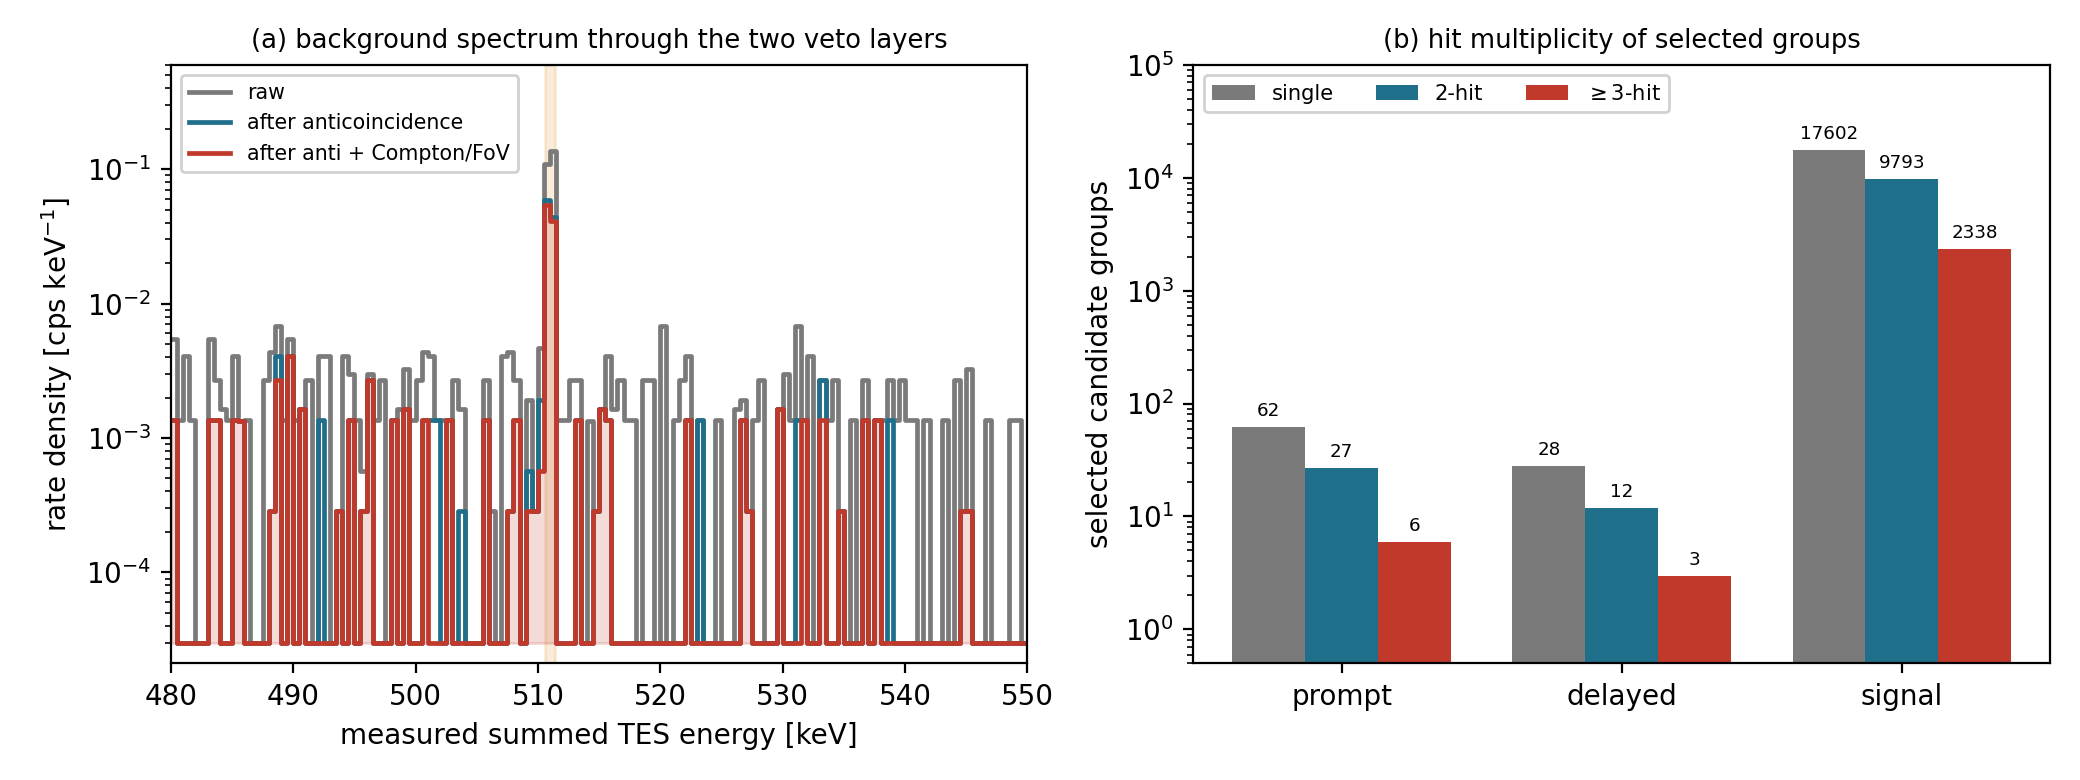
\includegraphics[width=\linewidth]{paper_source_figure_table/fig_s33_compton_multiplicity.png}
\caption{(a) Response-convolved background spectrum through the two veto layers
(raw; after anticoincidence; after anticoincidence$+$Compton/FoV). (b) Hit
multiplicity of the selected candidate groups per stream in the
$480$--$550\,\keV$ band. Absolute line-window rates are given in
Table~\ref{tab:phase2_cutflow}.}
\label{fig:s33_compton_mult}
\end{figure}

Unreconstructed events remain in the baseline rate accounting but are not
labelled as field-of-view-passing candidates. The role of multi-hit acceptance
can be quantified directly: a single-site-only selection would retain
$61.68\%$ of the focused-signal rate and $67.17\%$ of the selected background
rate in $\wii$, reducing the simple $S/\sqrt{B}$ figure to $0.753$ of the
baseline value. The adopted permissive multi-hit policy therefore preserves
statistical reach while using topology as a consistency veto rather than as an
imaging cut.

Table~\ref{tab:phase2_cutflow} summarizes the reference-geometry event flow with
the same TES energy window, CsI veto, and Compton/field-of-view test. The first
stage is the line-window sample before either veto, and the uncertainties are the
quadrature sums of the event-rate weights.

\begin{table}[t]
\centering
\caption{Reference-geometry event-level $\wii$ cut-flow. Focused-signal rates are normalized to a unit EventList input rate; the physical point-source rate is scaled separately.}
\label{tab:phase2_cutflow}
\footnotesize
{
\setlength{\tabcolsep}{3pt}
\begin{tabular}{p{0.20\linewidth}p{0.24\linewidth}p{0.08\linewidth}p{0.16\linewidth}p{0.20\linewidth}}
\toprule
Stream & Stage & Events & Rate / $\cps$ & Statistical uncertainty / $\cps$ \\
\midrule
Prompt background & Line-window pre-veto & 148 & $1.14624\times10^{-1}$ & $1.24549\times10^{-2}$ \\
Prompt background & After CsI veto & 68 & $4.61248\times10^{-2}$ & $5.59345\times10^{-3}$ \\
Prompt background & Topology/FOV selected & 63 & $4.27321\times10^{-2}$ & $5.38374\times10^{-3}$ \\
Delayed activation & Line-window pre-veto & 40 & $5.69229\times10^{-3}$ & $9.00030\times10^{-4}$ \\
Delayed activation & After CsI veto & 26 & $3.69999\times10^{-3}$ & $7.25627\times10^{-4}$ \\
Delayed activation & Topology/FOV selected & 26 & $3.69999\times10^{-3}$ & $7.25627\times10^{-4}$ \\
Focused signal & Line-window pre-veto & 28534 & $7.67167\times10^{-1}$ & $4.54160\times10^{-3}$ \\
Focused signal & After CsI veto & 28534 & $7.67167\times10^{-1}$ & $4.54160\times10^{-3}$ \\
Focused signal & Topology/FOV selected & 27993 & $7.52621\times10^{-1}$ & $4.49834\times10^{-3}$ \\
\bottomrule
\end{tabular}
\par}
\vspace{0.5ex}
\begin{minipage}{0.94\linewidth}
\footnotesize
The focused-signal rows report transfer rates for a unit EventList input rate
and show the survival fraction at each selection stage; the point-source signal rate in Table~\ref{tab:primary_sensitivity}
is scaled separately by the Laue effective area, reference flux, and atmospheric
transmission.
\end{minipage}
\end{table}

An independent topology benchmark uses the MEGAlib \texttt{revan} Compton event
reconstructor on 37,065 focused-signal events from a retained legacy geometry
\cite{Zoglauer2006}. Its energy-window population is not mixed with the
response-convolved reference-detector rate budget above; the benchmark is used
for interaction ordering and angular-resolution diagnostics. For two-hit
ordering it gives two quantitative results. First, the fraction of two-hit
events with at least one kinematically valid order is $100.0\%$
($10{,}421/10{,}421$), as expected analytically---for a fully absorbed
$511\keV$ two-hit event the scattered-photon energy cannot fall below the
$E_0/3$ Compton edge, so at least one order is always valid---confirming the
premise for retaining two-hit events. Second, the best order chosen by the
Klein--Nishina cross section with a kinematic quality factor agrees with the
order that points more nearly toward the source only $78.4\%$ of the time, so
committing to a single estimated order (as an imaging chain would) would use the
wrong Compton cone for about $22\%$ of two-hit events, whereas enumerating both
orders and accepting either field-of-view-consistent one avoids this
misassignment. The median $|\mathrm{ARM}|$ of in-window Compton events relative
to the true beam direction is about $24^\circ$ (two-hit $23.6^\circ$; three-hit
and higher $26.3^\circ$; only about $32\%$ have $|\mathrm{ARM}|<10^\circ$),
driven by the millimetre-scale scatter lever arms and pixel quantization; this
explains why the topology/field-of-view layer removes only about $10$--$14\%$ of
the background and cannot be sharpened into an imaging-level discriminant.
Finally, the fraction of unorderable events is very small (61 of 37,065, i.e.\
$0.16\%$, in \texttt{revan}; one in the analytic classifier), so the
unreconstructed class is a small boundary population.

\subsection{Mission-time trajectory and analytic rate folding}
\label{sec:mission_time_fold}

MeV balloon observations are background dominated: atmospheric secondaries and cosmic-ray-induced activation set the rate floor, and both respond to the flight environment \cite{Gallego2025Balloon,Kierans2017}. Detector-coupled Monte Carlo through a fixed mass model already provides the selected day-15 signal and background rates under a common veto and energy window (Sections~\ref{sec:background}--\ref{sec:selection}). Those rates, however, are defined at a single longitude, latitude, and altitude. On a multi-day float the residual atmospheric depth, geomagnetic cutoff, and activation inventory evolve, so a constant-rate extrapolation of the day-15 snapshot is not a substitute for a trajectory fold. As in other balloon MeV programmes (for example COSI's use of PARMA/EXPACS fields and time-dependent light curves along the flight \cite{Gallego2025Balloon}), we therefore introduce an analytic mission-time trajectory curve that maps the reference rates onto a continuous 20\,d performance estimate, and we test the fold with direct Cosima transports at selected trajectory states rather than re-running full statistics at every time bin.

The trajectory used here is a \emph{synthetic reference profile}, not balloon telemetry and not a source-visibility schedule. It comprises 81 bins from day~0 to day~20 (0.25\,d spacing) with a mild mid-latitude float envelope: altitude $h=38.75\pm2.5$\,km, latitude $34^\circ\pm0.25^\circ$, and longitude $100^\circ\pm0.25^\circ$, all phase-referenced to the day-15 anchor. Altitude is retained because zero-pressure-class and related long-duration balloons experience float-altitude excursions that change residual atmospheric depth by several $\mathrm{g\,cm^{-2}}$; depth controls both the atmospheric particle spectra that drive prompt background and activation, and the 511\,keV atmospheric transmission that multiplies the focused science rate. Latitude and longitude are retained only as a \emph{reference} geomagnetic/geographic modulation of cutoff rigidity on that same synthetic track; they do not encode Earth occultation, target elevation limits, or repointing losses. The resulting fold therefore supports a reference-exposure statistical sensitivity under a controlled trajectory envelope, not a flight forecast for a named launch campaign.

The analytic fold is defined by six physically separate layers. Atmospheric transmission multiplies only the celestial signal and does not rescale either the local particle field that drives prompt background and activation or the atmospheric-line source defined in Equation~\eqref{eq:atm511_flux}.

\emph{(1) Signal.} For a monochromatic point source with top-of-atmosphere flux $F_{511}$,
\begin{equation}
  R_{\mathrm{sig}}(t)=F_{511}\,A_{\mathrm{eff}}\,T_{\mathrm{atm},511}(t)\,\varepsilon_{\mathrm{det}},
  \label{eq:mission_signal}
\end{equation}
where $A_{\mathrm{eff}}$ is the on-axis Laue effective area, $T_{\mathrm{atm},511}(t)$ is the 511\,keV atmospheric transmission at the trajectory state, and $\varepsilon_{\mathrm{det}}$ collects detector and selection efficiency at the reference response. Relative to the day-15 anchor this is equivalent to
$S_{\mathrm{sig}}(t)=S_{15}\,T_{\mathrm{atm},511}(t)/T_{15,45}$ with
$T_{15,45}=0.6520$. In every bin the fixed $45^\circ$ elevation
($45^\circ$ zenith angle) gives
$T_{\mathrm{atm},511}(t)=\exp[-\mu_{\mathrm{air}}X_{\mathrm{vertical}}(t)/\cos45^\circ]$,
with $\mu_{\mathrm{air}}=0.08736\,\mathrm{cm^2\,g^{-1}}$. This uses the
slant column along the instrument axis and remains a fixed-axis reference rather
than a source-visibility calculation.

\emph{(2) Prompt background.} At particle-family resolution the selected prompt rate is the source--response sum
\begin{equation}
  R_{\mathrm{prompt},j}(t)=\sum_{b}\Phi_{b}(t)\,K_{j,b},
  \label{eq:prompt_source_response}
\end{equation}
where $b$ runs over atmospheric particle families (protons, neutrons, $e^{\pm}$, $\gamma$, $\mu^{\pm}$, \ldots), $\Phi_{b}(t)$ is the PARMA/EXPACS flux recalculated at the trajectory state, and $K_{j,b}$ is a detector response coefficient fixed once from the day-15 reference transport for selection $j$. Relative to the reference state this reweights family contributions by $\Phi_{b}(t)/\Phi_{b}(\mathrm{REF})$. Within a line window the same structure may be refined to $K_{b,E,\theta}$ when energy--angle response matrices are available.

\emph{(3) Atmospheric 511 keV line.} The separately transported day-15 line
response is scaled by the full-sphere line-integrated flux:
\begin{equation}
  R_{\mathrm{atm511},j}(t)=R_{\mathrm{atm511},j}(15)
  \frac{\Phi_{4\pi}(t)}{\Phi_{4\pi}(15)},\qquad
  R^{\mathrm{occ}}_{\mathrm{atm511}}(t)=R^{\mathrm{occ}}_{\mathrm{atm511}}(15)
  \frac{\Phi_{4\pi}(t)}{\Phi_{4\pi}(15)}.
  \label{eq:mission_atm511}
\end{equation}
Here $\Phi_{4\pi}(t)$ is evaluated from Equation~\eqref{eq:atm511_flux} along
the atmospheric-line proxy depth and rigidity curve, whose day-15 rigidity is
$11.0\,\mathrm{GV}$. This curve is distinct from the state-specific PARMA prompt
field, whose day-15 rigidity is $11.6\,\mathrm{GV}$. The total line flux is varied
while the transported day-15 angular response is held fixed; the line transport
is not rerun in every time bin.

\emph{(4) Activation production.} For each incident family $a$ and radioactive
source-parent nuclide $k$ in the final all-eight-family delayed inventory,
\begin{equation}
  P_{a,k}(t)=\Phi_{a}(t)\,Y_{a,k},
  \label{eq:activation_production}
\end{equation}
where $Y_{a,k}$ is the family-resolved yield fixed by the corresponding day-15
inventory and $\Phi_a(t)$ is the PARMA flux recalculated for that family at each
trajectory state. The $141.83\,\mathrm{Bq}$
all-family inventory of the mass-complete reference geometry is used for the
background-origin analysis, not substituted into this final-geometry fold; the
fold uses the final directionally graded configuration's
$36.4525153\,\mathrm{Bq}$ inventory.

\emph{(5) Delayed inventory.} With decay constant $\lambda_k$, each family--parent
inventory is advanced by
\begin{equation}
  N_{a,k}(t+\Delta t)=N_{a,k}(t)\,e^{-\lambda_k\Delta t}
  +\frac{P_{a,k}(t)}{\lambda_k}\bigl(1-e^{-\lambda_k\Delta t}\bigr),
  \qquad A_{a,k}(t)=\lambda_k N_{a,k}(t).
  \label{eq:delayed_inventory}
\end{equation}

\emph{(6) Delayed selected rate.}
\begin{equation}
  R_{\mathrm{delayed},j}(t)=\sum_{a}\sum_{k} A_{a,k}(t)\,\varepsilon_{j,a,k},
  \label{eq:delayed_selected}
\end{equation}
where $\varepsilon_{j,a,k}$ is the selected-rate response of source-parent
nuclide $k$ produced by family $a$ under selection $j$. A SIM IA INIT daughter
identity is retained as lineage evidence but does not replace the radioactive
source parent in this sum. Equations~\eqref{eq:mission_signal}--\eqref{eq:delayed_selected}
keep celestial transmission, prompt-particle modulation, atmospheric-line scaling,
activation production, and radioactive decay as separate physical steps.

To test the analytic predictions we select and hold fixed four trajectory
states---the day-15 reference (REF), a low-altitude early point (L1), a
high-altitude point (H1), and a low-altitude late point (L2)---and recalculate
PARMA spectra and Cosima atmospheric sources at those coordinates without using
the analytic scale as a free parameter. For a predicted scale $S^{\mathrm{pred}}$
from Equation~\eqref{eq:prompt_source_response} we report
\begin{equation}
  Q=\frac{R^{\mathrm{MC}}/R^{\mathrm{MC}}_{\mathrm{REF}}}{S^{\mathrm{pred}}}.
\end{equation}
Ideal agreement gives $Q\simeq1$. The final implementation applies separate
state-specific PARMA flux ratios to the day-15 response coefficient of each of the eight
prompt particle families and advances each retained delayed family--parent
nuclide with its matching family flux ratio. Direct trajectory transports validate the combined $e^+$,
$n$, and $\gamma$ modulation in the broad TES $480$--$550$\,keV band within
$2\sigma$ (maximum $|z|\simeq0.51$ across the off-reference points); for the
high-statistics $e^+$ band alone, $Q$ follows the recalculated PARMA $e^+$ flux
scale to within about $1\%$. These multi-point results directly validate the tested families,
while the other prompt-family modulation remains an analytic source-field
reweighting; all final 511 keV-window response coefficients are supplied by the
day-15 detector chain.

With the final-geometry day-15 rates fixed by the full detector chain, these trajectory
scales provide $S(t)$, $B(t)$, and the cumulative counts in
Equation~\eqref{eq:cumulative_counts}. Section~\ref{sec:results} presents the
resulting central curve and conditional componentwise transport-counting endpoint together, so
the reader can see both the expected mission performance and the effect of limited
Monte Carlo support on the same time axis.


\section{Results}
\label{sec:results}

\subsection{What sets the 511 keV line-window background?}
\label{subsec:reference_background_results}

The mass-complete reference calculation tells us which interactions must be
controlled before a shield is specified. In the $510.58$--$511.42\keV$ window,
the common response, active-veto, and topology/field-of-view selection leaves 63 prompt and
26 delayed Monte Carlo records. Because the streams represent different physical
exposures, their weights differ; the selected records correspond to a
prompt-plus-delayed diagnostic rate of
$(4.64320\pm0.54324)\times10^{-2}\cps$. Table~\ref{tab:reference_background_budget}
gives both the record counts and the weighted rates. The separately transported
atmospheric 511\,keV line is not included in this reference-geometry diagnostic.

\begin{table}[t]
\centering
\caption{Prompt-plus-delayed primary-window diagnostic for the reference detector; the separately transported atmospheric 511\,keV line is not included. Relative uncertainties are Monte Carlo counting standard errors. Counts from independently normalized components are not directly proportional to their rate contributions.}
\label{tab:reference_background_budget}
\footnotesize
\resizebox{\linewidth}{!}{%
\begin{tabular}{lrrrrrl}
\toprule
Component & Selected records & Rate / $\cps$ & MC $\sigma$ / $\cps$ & Relative MC $\sigma$ / \% & Total rate / \% & Selected-event origin \\
\midrule
Prompt $e^+$ & 43 & $2.91730\times10^{-2}$ & $4.44885\times10^{-3}$ & 15.2 & 62.83 & incident-family tag \\
Prompt $n$ & 18 & $1.22099\times10^{-2}$ & $2.87791\times10^{-3}$ & 23.6 & 26.30 & incident-family tag \\
Prompt $\mu^+$ & 2 & $1.34910\times10^{-3}$ & $9.53958\times10^{-4}$ & 70.7 & 2.91 & incident-family tag \\
Prompt subtotal & 63 & $4.27321\times10^{-2}$ & $5.38374\times10^{-3}$ & 12.6 & 92.03 & eight-family transport \\
Delayed activation & 26 & $3.69999\times10^{-3}$ & $7.25627\times10^{-4}$ & 19.6 & 7.97 & 24 $^{64}$Cu, 2 $^{61}$Cu \\
\midrule
Total & 89 & $4.64320\times10^{-2}$ & $5.43242\times10^{-3}$ & 11.7 & 100.00 & prompt plus delayed \\
\bottomrule
\end{tabular}}
\end{table}

\begin{figure}[t]
\centering
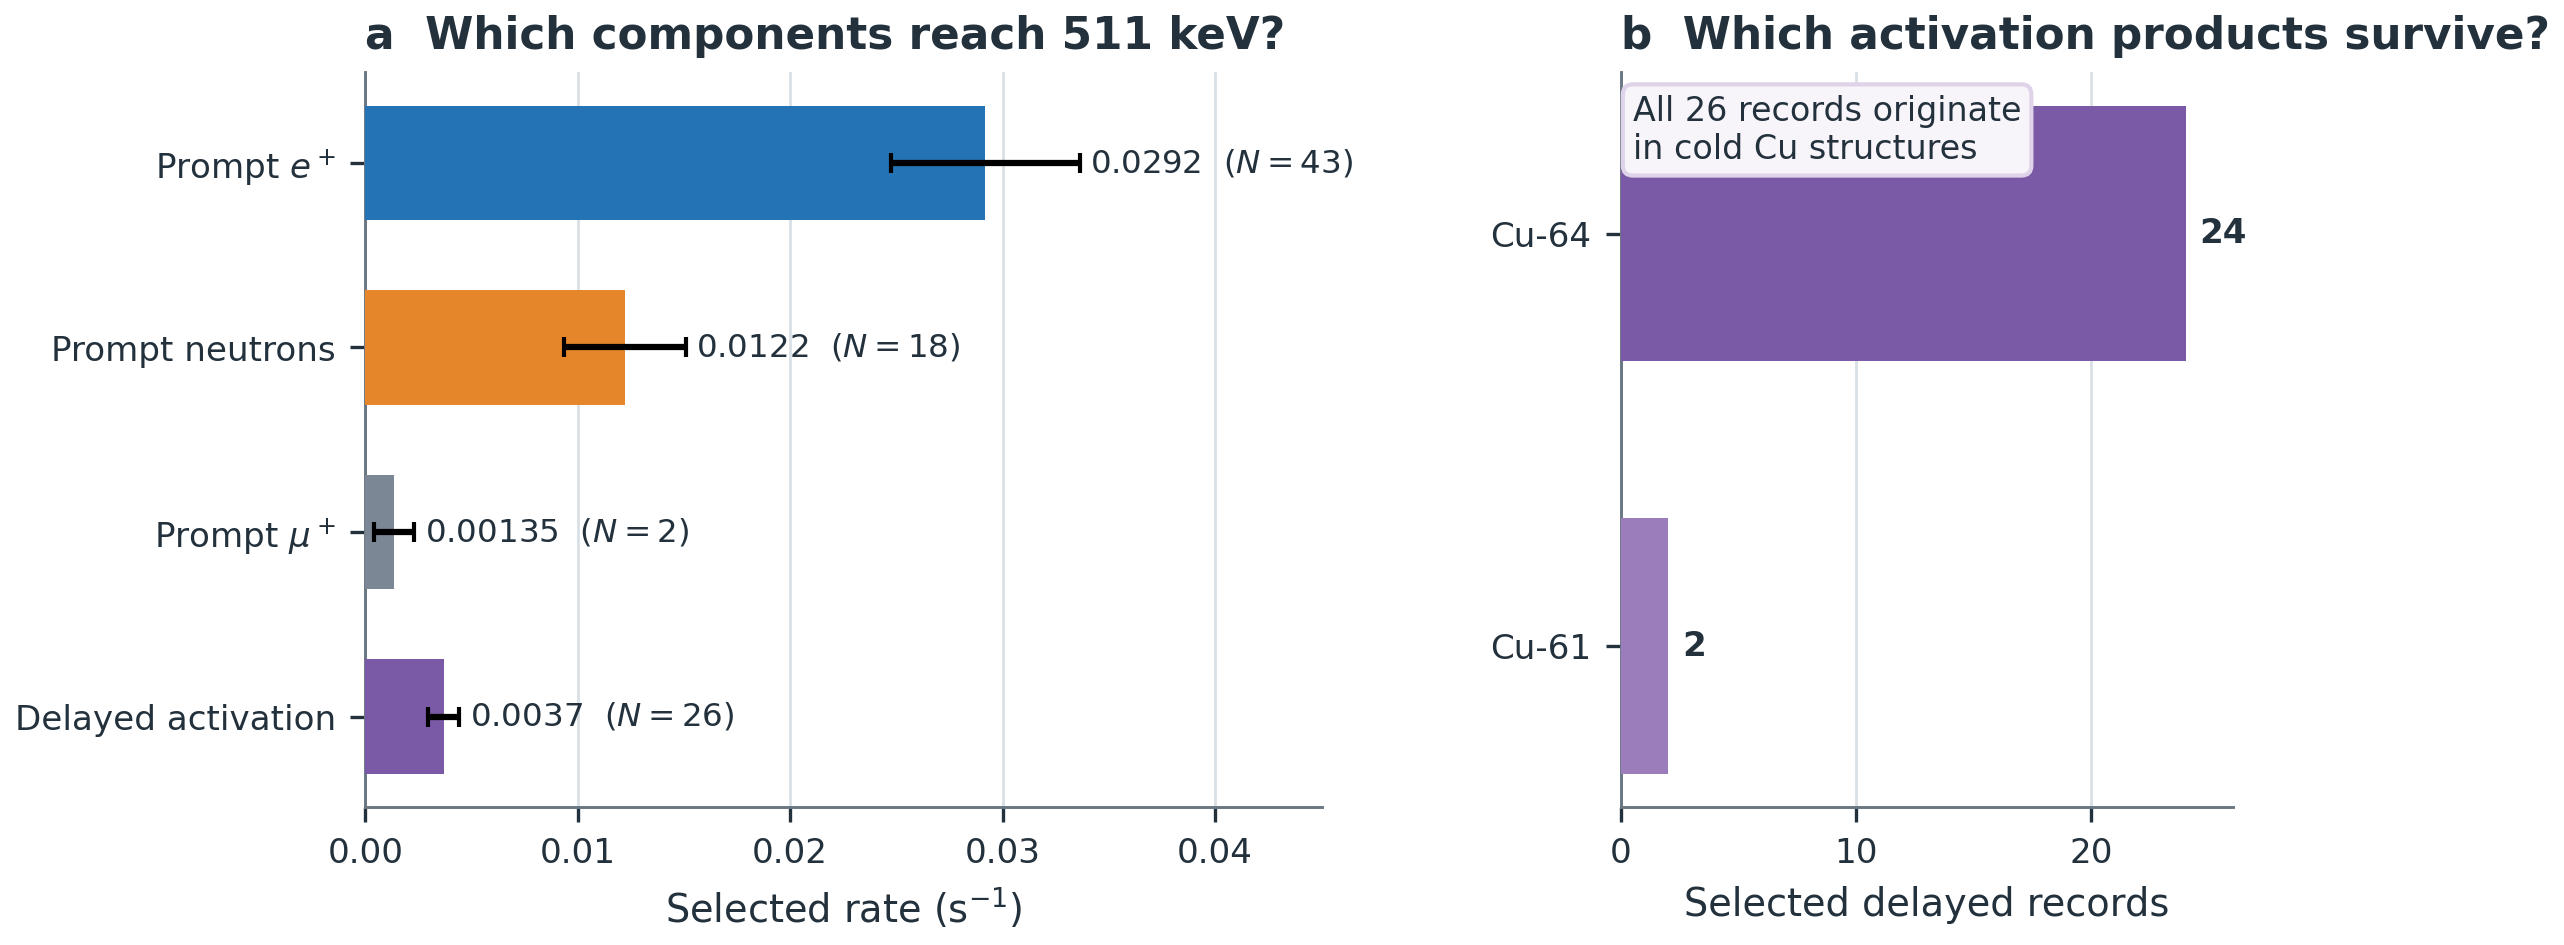
\includegraphics[width=0.98\linewidth]{paper_source_figure_table/fig_background_origin_story.png}
\caption{Physical origin of the selected prompt-plus-delayed diagnostic background
in the mass-complete reference geometry; the atmospheric 511\,keV line is not
included. (a) Weighted rate by prompt particle family and
delayed activation; error bars are Monte Carlo counting standard errors from
Equation~\eqref{eq:weighted_rate_stats}. (b) Parent isotope of the 26 selected
delayed records. Positrons and neutrons provide $89.13\%$ of the total selected
rate, while the delayed records all originate in cold copper structures.}
\label{fig:background_origin_story}
\end{figure}

Figure~\ref{fig:background_origin_story} makes the prompt result easy to read.
Incident positrons contribute $2.917\times10^{-2}\cps$ and neutrons contribute
$1.221\times10^{-2}\cps$. Together they supply $96.84\%$ of the prompt rate
and $89.13\%$ of the prompt-plus-delayed diagnostic budget. The atmospheric
511\,keV line is carried as the separate component defined in
Section~\ref{subsec:atm511_source}; under the adopted detector response and line
window it is not spectrally distinguishable from the science line.
All eight prompt families remain in the final transport; the decomposition is used
to understand the physics, not to remove source classes from the calculation.

The delayed events show a different source-level and detector-selected
distribution. Of the corrected $141.83$ Bq day-15 inventory, neutron-induced
products contribute $94.25\%$ and $\mu^-$-induced products $5.38\%$. The source
activity is distributed mainly among CsI ($63.08\%$), outer mechanical
structures ($15.71\%$), and cold plates ($9.43\%$); the neutron and $\mu^-$
material distributions have $D_{\mathrm{TV}}=0.823$. After detector response and
selection, 24 of the 26 line-window records are $^{64}$Cu decays and the other
two are $^{61}$Cu decays, all in cold copper structures near the TES. The
source inventory and selected line-window background therefore identify
different material priorities: active coverage controls the dominant prompt and
atmospheric paths, while copper close to the focal plane supplies the local
delayed component.

The final directionally graded configuration uses a separate all-eight-family
activation calculation.
Its NUBASE-corrected day-15 activity is $36.4525153\,\mathrm{Bq}$: neutron,
$\mu^-$, proton, and $\alpha$ production contribute $83.83\%$, $10.82\%$,
$4.64\%$, and $0.69\%$, respectively, with smaller positive $e^+$, $\gamma$,
and $\mu^+$ inventories; $e^-$ is the finite-BUILDUP zero observation. The 78
final delayed records are carried by 60 neutron, 12 proton, five $\mu^-$, and one
$\alpha$ event. Their time fold is resolved jointly by incident family and
exact-source parent nuclide. In particular, the one SIM lineage that starts as
$^{182}$W is assigned to its position-matched radioactive $^{182}$Ta source
parent rather than treating stable ground-state $^{182}$W as an activity.

\FloatBarrier

\subsection{Final directionally graded active-shield geometry}
\label{subsec:optimized_shield_results}

The final active shield converts the background map into a simple geometry. The side
is the most important active surface because it surrounds the long cryostat wall
and the side optical opening, so it retains 40 mm BGO coverage. The bottom uses a
30 mm BGO disk, while the top uses a 10 mm annulus around the service opening.
The focused beam still enters through the aligned side aperture. A thin Al/Kapton
outer enclosure remains, with no continuous external W layer.
Figure~\ref{fig:optimized_shield_background} connects this layout to the event
selection and final background budget; Table~\ref{tab:final_geometry} lists the
dimensions. These values define the only optimized geometry used in the following
full-chain and mission calculations.

\begin{figure}[!ht]
\centering
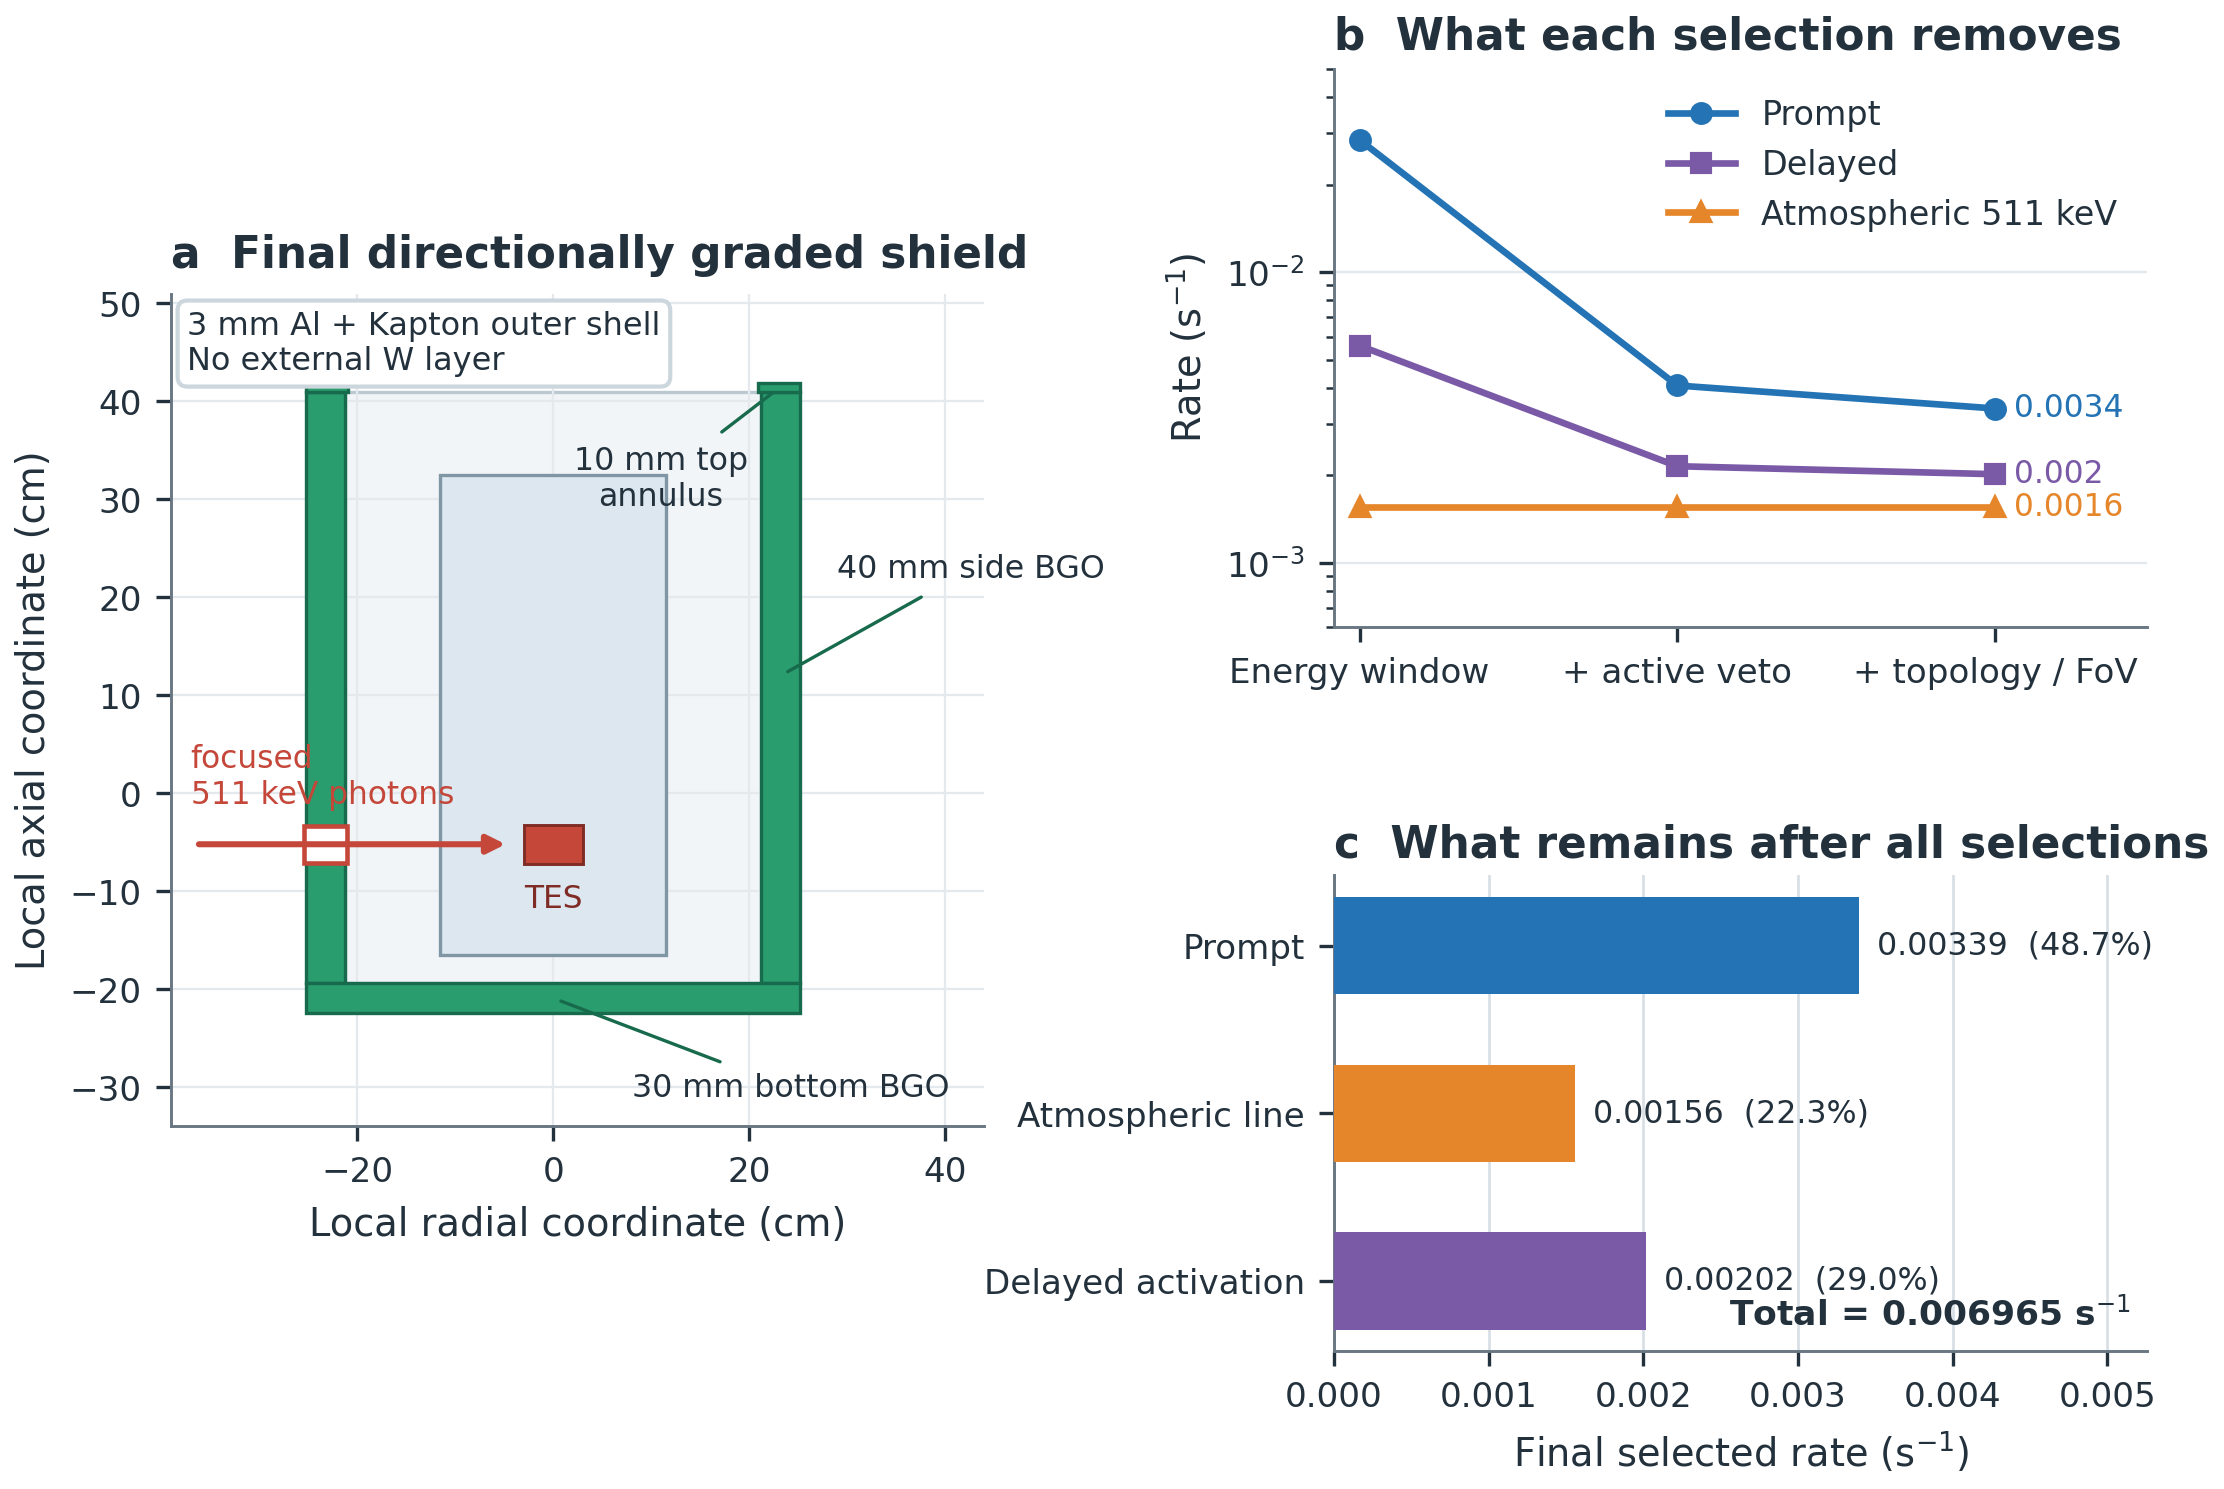
\includegraphics[width=0.90\linewidth]{paper_source_figure_table/fig_optimized_shield_background.png}
\caption{From the final graded-shield geometry to the selected background. (a) Cross-section
of the directionally graded BGO shield; dimensions are read from the generated
geometry manifest. The cryostat and TES symbols are simplified only to expose the
shield layout and side beam path. (b) Prompt, delayed, and atmospheric-line rates
after the energy window, active veto, and topology/field-of-view selection.
(c) Composition of the final, response-convolved
$6.96486\times10^{-3}\cps$ background.}
\label{fig:optimized_shield_background}
\end{figure}

\begin{table}[!ht]
\centering
\caption{Final directionally graded active-shield geometry. Radial and axial coordinates are local to the detector--cryostat frame.}
\label{tab:final_geometry}
\footnotesize
\begin{tabular}{p{0.22\linewidth}p{0.33\linewidth}p{0.36\linewidth}}
\toprule
Element & Final setting & Physical role \\
\midrule
Side BGO & 40 mm; $r=21.2$--25.2 cm, $z=-19.4$--40.9 cm & Continuous active coverage around the long side wall while preserving the optical cut \\
Bottom BGO & 30 mm; $r=0$--25.2 cm, $z=-22.4$--$-19.4$ cm & Active coverage of the lower end surface \\
Top BGO & 10 mm annulus; $r=20.9$--25.2 cm, $z=40.9$--41.9 cm & Covers the outer top edge while leaving the central service opening \\
Side optical path & Existing Boolean aperture and aligned Al/Be windows plus W collimator & Carries the focused 511 keV beam to the TES array \\
Outer enclosure & 3 mm Al plus Kapton; no continuous external W layer & Mechanical envelope and electrical insulation \\
BGO offline anticoincidence & $E_{\mathrm{sh}}^{(c)}<50$ keV & Event-by-event sum of recorded energy deposits in the active BGO volumes \\
\bottomrule
\end{tabular}
\end{table}

The resulting shield is directional rather than uniform: it places the deepest
active layer around the side and uses smaller end layers where the geometry has a
shorter exposed path. This design also keeps the optical route easy to read: the
collimator remains a local element in the beam path, whereas the outer enclosure
does not add a second continuous high-$Z$ layer. The geometry drawing, cut-flow,
and component budget are therefore three linked views of the same final design.

\FloatBarrier

\subsection{Full-chain background and statistical support}
\label{subsec:optimized_fullchain}

Table~\ref{tab:optimized_cutflow} follows each final-geometry stream through the same event
sequence shown in Figure~\ref{fig:optimized_shield_background}b. ``Pre-veto''
means that the TES energy already lies in the primary line window. Record counts
show the Monte Carlo support at each step; final rates give the physical result
after the different source exposures have been applied.

\begin{table}[!ht]
\centering
\caption{Response-convolved primary-window cut-flow for the final graded-shield geometry at the day-15 reference state. The signal rate is scaled to $\fzero=10^{-4}\phcms$; background fractions use the total final background rate.}
\label{tab:optimized_cutflow}
\footnotesize
\resizebox{\linewidth}{!}{%
\begin{tabular}{lrrrrrrr}
\toprule
Stream & Pre-veto records & Active-veto pass & Final records & Active survival / \% & Topology survival / \% & Final rate / $\cps$ & Background / \% \\
\midrule
Eight-family prompt & 42 & 6 & 5 & 14.29 & 83.33 & $3.39303\times10^{-3}$ & 48.72 \\
All-eight-family delayed & 346 & 83 & 78 & 38.49 & 93.88 & $2.01657\times10^{-3}$ & 28.95 \\
Atmospheric 511\,keV line & 8 & 8 & 8 & 100.00 & 100.00 & $1.55526\times10^{-3}$ & 22.33 \\
Focused signal & 28566 & 28566 & 28010 & 100.00 & 98.05 & $9.86228\times10^{-4}$ & -- \\
\midrule
Total background & 396 & 97 & 91 & -- & -- & $6.96486\times10^{-3}$ & 100.00 \\
\bottomrule
\end{tabular}}
\end{table}

The active shield does most of the prompt rejection. It lowers the response-convolved
line-window prompt rate from $2.84914\times10^{-2}$ to
$4.07188\times10^{-3}\cps$, so only $14.29\%$ survives that stage. The topology/field-of-view test then lowers
it to $3.39303\times10^{-3}\cps$. For delayed activation, the corresponding
rates are $5.58116\times10^{-3}$, $2.14813\times10^{-3}$, and
$2.01657\times10^{-3}\cps$; because the delayed families have different event
weights, the active and topology survivals in Table~\ref{tab:optimized_cutflow}
are rate ratios (38.49\% and 93.88\%), not record-count ratios. Before detector-response
convolution, nine transported atmospheric-line records lay in the primary window.
After the independent 420\,eV FWHM per-pixel response and the 0.3\,keV measured-hit
threshold were applied, eight remained in the measured window. No atmospheric-line
pixel hit was removed by the threshold in this response realization; one
response-convolved event instead moved below the lower window boundary.
All eight measured-window records pass the active veto and topology test, leaving
the rate unchanged at $1.55526\times10^{-3}\cps$ through those two selection stages;
under the adopted energy and topology observables, a 511\,keV photon entering
through the open path is not distinguishable from a source photon. The focused
signal behaves differently:
all 28566 line-window records pass the active veto, and 28010 ($98.05\%$) pass the
final topology test.

At the day-15 reference state, after all selections, prompt particles contribute
$48.72\%$ of the background, the atmospheric line $22.33\%$, and delayed
activation $28.95\%$. Thus the active
shield removes most prompt and delayed events accompanied by shield energy without
rejecting the focused beam, while the remaining budget naturally becomes a mixture
of prompt leakage, a line-like atmospheric term, and local activation.

The five final prompt records comprise two $e^+$ and three neutron records. The
other six prompt families have zero selected records in the available sample.
Table~\ref{tab:optimized_component_precision} retains those zeros and their
different event weights, because zero selected records give a rate upper limit.
The photon family has the largest event weight and therefore sets most of the
conditional componentwise prompt endpoint.

\begin{table}[!ht]
\centering
\caption{Transport-counting precision of the optimized day-15 final background. For components with defined transport exposure, intervals are two-sided 95\% Garwood intervals scaled by the listed event weight. Subtotal and total upper values are componentwise endpoint sums, not a joint-coverage interval or detector systematic uncertainty. The finite-BUILDUP $e^-$ zero has no fictitious exposure or Garwood endpoint.}
\label{tab:optimized_component_precision}
\footnotesize
\resizebox{\linewidth}{!}{%
\begin{tabular}{lrrrrr}
\toprule
Component & Final records & Weight / $\cps$ & Central rate / $\cps$ & Exact 95\% rate interval / $\cps$ & Total central / \% \\
\midrule
Prompt $\alpha$ & 0 & $6.78971\times10^{-4}$ & 0 & $[0,2.50464\times10^{-3}]$ & 0 \\
Prompt $e^-$ & 0 & $6.78761\times10^{-4}$ & 0 & $[0,2.50387\times10^{-3}]$ & 0 \\
Prompt $e^+$ & 2 & $6.78847\times10^{-4}$ & $1.35769\times10^{-3}$ & $[1.64423\times10^{-4},4.90446\times10^{-3}]$ & 19.49 \\
Prompt $\gamma$ & 0 & $5.42680\times10^{-3}$ & 0 & $[0,2.00188\times10^{-2}]$ & 0 \\
Prompt $\mu^-$ & 0 & $6.77164\times10^{-4}$ & 0 & $[0,2.49798\times10^{-3}]$ & 0 \\
Prompt $\mu^+$ & 0 & $6.77705\times10^{-4}$ & 0 & $[0,2.49997\times10^{-3}]$ & 0 \\
Prompt $n$ & 3 & $6.78446\times10^{-4}$ & $2.03534\times10^{-3}$ & $[4.19736\times10^{-4},5.94812\times10^{-3}]$ & 29.22 \\
Prompt $p$ & 0 & $6.77234\times10^{-4}$ & 0 & $[0,2.49824\times10^{-3}]$ & 0 \\
Prompt subtotal & 5 & -- & $3.39303\times10^{-3}$ & upper sum: $4.33761\times10^{-2}$ & 48.72 \\
Delayed $\alpha$ & 1 & $3.48183\times10^{-7}$ & $3.48183\times10^{-7}$ & $[8.81522\times10^{-9},1.93995\times10^{-6}]$ & 0.005 \\
Delayed $e^-$ & 0 & -- & 0 & finite-BUILDUP zero; no interval & 0 \\
Delayed $e^+$ & 0 & $2.15006\times10^{-9}$ & 0 & $[0,7.93131\times10^{-9}]$ & 0 \\
Delayed $\gamma$ & 0 & $5.46390\times10^{-9}$ & 0 & $[0,2.01557\times10^{-8}]$ & 0 \\
Delayed $\mu^-$ & 5 & $4.20909\times10^{-6}$ & $2.10454\times10^{-5}$ & $[6.83339\times10^{-6},4.91130\times10^{-5}]$ & 0.30 \\
Delayed $\mu^+$ & 0 & $7.94287\times10^{-10}$ & 0 & $[0,2.93003\times10^{-9}]$ & 0 \\
Delayed $n$ & 60 & $3.28039\times10^{-5}$ & $1.96823\times10^{-3}$ & $[1.50197\times10^{-3},2.53351\times10^{-3}]$ & 28.26 \\
Delayed $p$ & 12 & $2.24533\times10^{-6}$ & $2.69439\times10^{-5}$ & $[1.39223\times10^{-5},4.70656\times10^{-5}]$ & 0.39 \\
Delayed subtotal & 78 & -- & $2.01657\times10^{-3}$ & upper sum: $2.63166\times10^{-3}$ & 28.95 \\
Atmospheric 511\,keV line & 8 & $1.94408\times10^{-4}$ & $1.55526\times10^{-3}$ & $[6.71451\times10^{-4},3.06448\times10^{-3}]$ & 22.33 \\
\midrule
Total background & 91 & -- & $6.96486\times10^{-3}$ & componentwise upper endpoint: $4.90722\times10^{-2}$ & 100.00 \\
\bottomrule
\end{tabular}}
\end{table}

The 64 deterministic response seeds provide a separate numerical-integration
check. Their day-15 background has mean
$6.94643\times10^{-3}\cps$ and sample standard deviation
$3.89046\times10^{-4}\cps$; the prespecified primary-seed value
$6.96486\times10^{-3}\cps$ differs from that mean by $0.047$ sample standard
deviations. We therefore use the fixed-seed value for the primary result
and keep the response-seed ensemble distinct from the conditional componentwise
transport-counting endpoint in Table~\ref{tab:optimized_component_precision}.

\FloatBarrier

\subsection{Mission performance of the final geometry}
\label{subsec:final_mission_performance}

The final rates were folded through all 81 trajectory bins. The accidental-coincidence
live factor remains between 0.97165 and 0.97985. At 20 d, the central curve contains
1650.29 focused-signal counts and 11789.08 background counts, giving
$Z=15.199$. Figure~\ref{fig:optimized_mission_significance} shows how the
significance accumulates rather than reporting only the endpoint.

\begin{figure}[!ht]
\centering
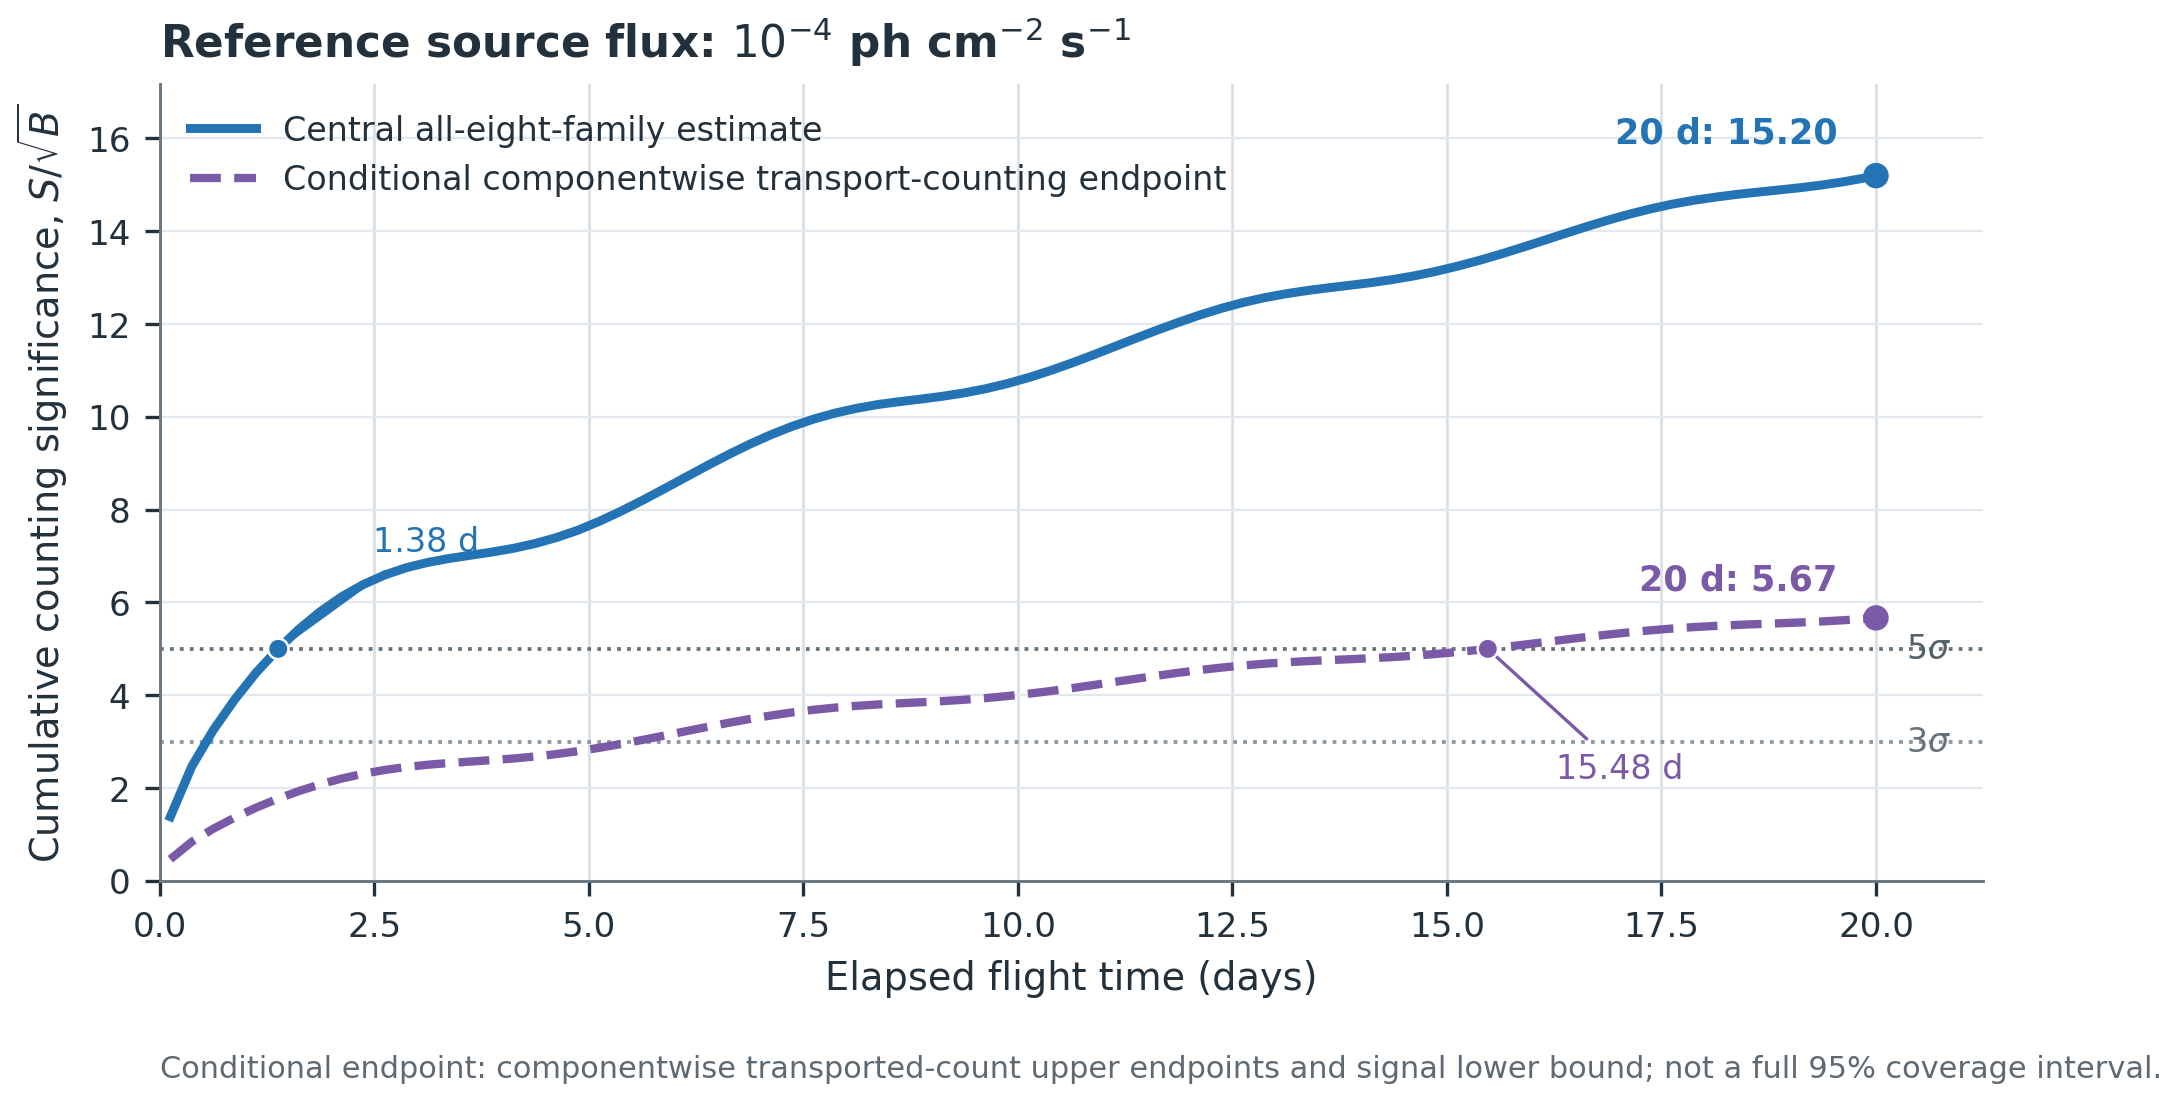
\includegraphics[width=0.98\linewidth]{paper_source_figure_table/fig_optimized_mission_significance.png}
\caption{Cumulative counting significance of the final graded-shield geometry for a continuously observed
$10^{-4}\phcms$ point source along the 20 d reference trajectory. The solid
curve uses the central selected rates. The dashed curve uses the upper exact
95\% counting endpoints for every background component and the lower exact
95\% signal-acceptance endpoint. Their componentwise combination is conditional,
not a joint 95\% interval. The curves reach $5\sigma$ at 1.38 and
15.48 d, respectively, and end at 15.20 and 5.67.}
\label{fig:optimized_mission_significance}
\end{figure}

\begin{table}[!ht]
\centering
\caption{Final graded-shield mission projection. The endpoint column propagates componentwise Garwood background upper endpoints and the Clopper--Pearson signal lower endpoint through the same trajectory. It is conditional on the transported samples and selected family--nuclide mixture and is not a joint-coverage interval.}
\label{tab:primary_sensitivity}
\footnotesize
\begin{tabular}{lrr}
\toprule
Quantity & Central estimate & Conditional componentwise transport-counting endpoint \\
\midrule
Day-15 background / $\cps$ & $6.96486\times10^{-3}$ & $4.90722\times10^{-2}$ \\
Day-15 signal at $\fzero$ / $\cps$ & $9.86228\times10^{-4}$ & $9.80445\times10^{-4}$ \\
$T_{3\sigma}$ / d & 0.545 & 5.519 \\
$T_{5\sigma}$ / d & 1.382 & 15.476 \\
$Z_{20\mathrm{d}}$ & 15.199 & 5.667 \\
$\fthree(20\,\mathrm{d})$ / $\phcms$ & $1.9738\times10^{-5}$ & $5.2934\times10^{-5}$ \\
\bottomrule
\end{tabular}
\end{table}

The two columns answer two useful questions. The central estimate is the expected
result from the simulated rates: it reaches $3\sigma$ in 0.545 d, $5\sigma$ in
1.382 d, and a 20 d flux threshold of $1.9738\times10^{-5}\phcms$. The
conditional endpoint asks how the answer changes if every transported background
component is moved to its exact upper counting endpoint and the signal acceptance
to its lower endpoint. It reaches $5\sigma$ in 15.476 d and gives a 20 d threshold
of $5.2934\times10^{-5}\phcms$. This endpoint does not have 95\% joint coverage:
the componentwise sum has no joint-coverage guarantee and omits finite-BUILDUP
zero-family, finite-$M$ source sampling, and nuclide-mixture uncertainty. The large separation between the curves is driven
mainly by the zero-count, high-weight prompt-photon component in
Table~\ref{tab:optimized_component_precision}; it shows exactly where additional
Monte Carlo statistics would most improve the precision of the prediction.

\section{Discussion}
\label{sec:discussion}

The main result is a connected physical explanation of the final design. In the
reference geometry, positrons and neutrons dominate the selected prompt rate, while
the selected activation events come from copper close to the TES rather than from
the volumes with the largest total activity. The final graded-shield geometry responds to the
first pattern with deep side BGO coverage and treats the second as a local activation
term in the same detector selection. At the day-15 reference state, after the
common veto and topology test, the background is $6.965\times10^{-3}\cps$ and
the focused signal retains $98.05\%$
of its line-window records. The geometry, background budget, and mission curve are
therefore three views of the same result.

This analysis sequence is consistent with methods used in recent
instrument-background studies.
COSI builds its balloon background from the transported payload, separates prompt
and activation components, and compares their spectral and time behaviour with
flight data \cite{Gallego2025Balloon}. DIXE likewise begins with a detailed TES
payload model and asks which incident particles, production regions, and processes
make the detected spectrum \cite{Tian2026DIXE}. In our case that decomposition is
especially important because source inventory and selected line-window background
lead to different answers: $^{128}$I dominates the reference activity, but cold-Cu
isotopes dominate the selected delayed records. Designing from selected events
rather than from inventory alone keeps the optimization tied to the science window.

The final component mix also shows what each instrument layer contributes. Active
BGO removes most prompt and delayed events that are accompanied by shield energy.
The topology test provides a smaller additional reduction while retaining nearly
all focused events. The atmospheric 511 keV component survives because it is
degenerate with the source in the present energy and single-photon-topology
observables. Its $22.33\%$ share at the
day-15 reference state is not a failure of anticoincidence; it is a
direction-dependent, full-sphere atmospheric-line background component that must
be carried through the trajectory. Its separability from source emission remains
to be tested with future pointing and control-region analyses.

The observing role of this telescope is complementary to INTEGRAL/SPI and COSI,
which measure the diffuse bulge, disk, and broader Galactic emission
\cite{Siegert2016AA,Kierans2020,Siegert2020COSI,Yoneda2025,Karwin2023}.
The Laue-lens TES concept exchanges sky coverage for a concentrated beam and a
sub-keV window. Its natural targets are compact 511 keV sources, an unresolved
central component, and pointed follow-up observations. The 20 d values in
Table~\ref{tab:primary_sensitivity} quantify that narrow-line, continuously
observed reference case.

\subsection{Scope and next steps}
\label{subsec:limitations}

The mission values are statistical projections for the engineering
detector--cryostat geometry and the synthetic, continuously on-source trajectory.
They use a 50 keV offline BGO deposited-energy veto, a detector-level topology
test, and all-eight-family activation in
the final delayed stream. Seven families have positive delayed transports; $e^-$
is a finite-BUILDUP zero observation, not a physical-zero claim. The veto is
applied to the event-wise sum of recorded shield deposits in post-processing.
It is an ideal deposited-energy threshold, not a threshold derived from a modeled
BGO hardware trigger-efficiency curve. The present background budget covers only
the detector--cryostat mass-model branch; background from the Laue optics and
balloon platform is outside this calculation. These choices define the calculation
represented by the central curve and conditional componentwise transport-counting
endpoint. The latter is neither a joint 95\% coverage interval nor a treatment
of radiation-field, cross-section, finite-$M$, nuclide-mixture, calibration, or
reconstruction systematics.

The atmospheric-line contribution has additional source-model limitations. The
reported result uses the nominal normalization, rigidity and depth scaling, and
the semi-empirical downward angular kernel of Section~\ref{subsec:atm511_source}.
The smooth EXPACS/PARMA continuum was not line-subtracted, so unresolved overlap
with the separately transported line remains a recognized but unquantified
source-model uncertainty. The mission fold also
scales the total line flux while retaining the transported day-15 angular
response, without a new Cosima transport in each time bin. These effects are not
included in the conditional componentwise transport-counting endpoint.

The next validation can focus on the terms that matter most in the figures: increase
the prompt-photon exposure that controls the conditional endpoint, repeat the
all-family activation position sampling to quantify finite-$M$ convergence, replace the reference trajectory
with a flight plan and visibility history, and calibrate the energy response and veto
thresholds in the final detector design. A spatial--spectral likelihood can then use
the focused spot and control regions while profiling background nuisance parameters
\cite{Cowan2011}. This sequence extends the present component model without
changing its source-to-geometry logic.

\subsection{Conclusions}
\label{sec:conclusions}

The mass-complete reference geometry shows where the focused beam, TES array,
cold copper, and active shield meet. Its selected-event map identifies positrons and
neutrons as the main prompt sources and cold-Cu isotopes as the delayed line-window
source. Those findings lead to the final directionally graded BGO shield with
40/30/10 mm side/bottom/top coverage. At the day-15 reference state, the
final-geometry full chain gives
$B=6.965\times10^{-3}\cps$ and $S=9.862\times10^{-4}\cps$ at the
top-of-atmosphere reference flux $\fzero=10^{-4}\phcms$. Over the fixed-$45^\circ$-elevation,
20 d reference trajectory, the central and conditional componentwise
transport-counting results reach $Z=15.20$ and 5.67, corresponding to
$3\sigma$ thresholds of $1.974\times10^{-5}$ and
$5.293\times10^{-5}\phcms$. The result demonstrates how a particle- and
material-resolved background model can be turned into a clear final geometry and
a mission-scale 511 keV performance prediction.

\section*{Data and software availability}
Before publication, a versioned public repository or institutional archive should provide the geometry and source definitions, random seeds, analysis and figure-generation scripts, LaTeX source, and derived validation products needed to reproduce the tables and figures in this paper.

\section*{Declarations}
\textbf{Funding} To be completed before journal submission.

\textbf{Competing interests} To be completed before journal submission.

\textbf{Author contributions} To be completed before journal submission.

\textbf{Ethics approval and consent to participate} Not applicable.

\begin{thebibliography}{99}

\bibitem{Prantzos2011}
N. Prantzos, C. Boehm, A.M. Bykov, R. Diehl, K. Ferriere, N. Guessoum, P. Jean, J. Knoedlseder, A. Marcowith, I.V. Moskalenko, A. Strong, G. Weidenspointner, The 511 keV emission from positron annihilation in the Galaxy, Rev. Mod. Phys. 83 (2011) 1001--1056, doi:10.1103/RevModPhys.83.1001.

\bibitem{Jean2006}
P. Jean, J. Knoedlseder, V. Lonjou, M. Allain, J.-P. Roques, G.K. Skinner, B.J. Teegarden, G. Vedrenne, P. von Ballmoos, B. Cordier, P. Caraveo, R. Diehl, P. Durouchoux, P. Leleux, R. Schanne, G. Weidenspointner, Spectral analysis of the Galactic $e^+e^-$ annihilation emission, Astron. Astrophys. 445 (2006) 579--589, doi:10.1051/0004-6361:20053765.

\bibitem{Kierans2020}
C.A. Kierans, S.E. Boggs, A. Zoglauer, A.W. Lowell, C. Sleator, J. Beechert, T.J. Brandt, P. Jean, H. Lazar, J. Roberts, T. Siegert, J.A. Tomsick, P. von Ballmoos, Detection of the 511 keV Galactic positron annihilation line with COSI, Astrophys. J. 895 (2020) 44, doi:10.3847/1538-4357/ab89a9.

\bibitem{Siegert2016AA}
T. Siegert, R. Diehl, G. Khachatryan, M.G.H. Krause, F. Guglielmetti, J. Greiner, A.W. Strong, X. Zhang, Gamma-ray spectroscopy of positron annihilation in the Milky Way, Astron. Astrophys. 586 (2016) A84, doi:10.1051/0004-6361/201527510.

\bibitem{Siegert2016V404}
T. Siegert, R. Diehl, J. Greiner, M.G.H. Krause, A.M. Beloborodov, M. Cadolle Bel, F. Guglielmetti, J. Rodriguez, A.W. Strong, X. Zhang, Positron annihilation signatures associated with the outburst of the microquasar V404 Cygni, Nature 531 (2016) 341--343, doi:10.1038/nature16978.

\bibitem{Knodlseder2005AllSky}
J. Knoedlseder, P. Jean, V. Lonjou, G. Weidenspointner, N. Guessoum, R. Diehl, W. Gillard, M.J. Harris, G.K. Skinner, P. von Ballmoos, G. Vedrenne, P. Caraveo, B. Cordier, V. Schoenfelder, B.J. Teegarden, The all-sky distribution of 511 keV electron-positron annihilation emission, Astron. Astrophys. 441 (2005) 513--532, doi:10.1051/0004-6361:20042063.

\bibitem{Yoneda2025}
H. Yoneda, T. Siegert, S. Mittal, Imaging the positron annihilation line with 20 years of INTEGRAL/SPI observations, arXiv:2509.01066, 2025.

\bibitem{Siegert2020COSI}
T. Siegert, S.E. Boggs, J.A. Tomsick, A.C. Zoglauer, C.A. Kierans, C.C. Sleator, J. Beechert, T.J. Brandt, P. Jean, H. Lazar, A.W. Lowell, J.M. Roberts, P. von Ballmoos, Imaging the 511 keV positron annihilation sky with COSI, Astrophys. J. 897 (2020) 45, doi:10.3847/1538-4357/ab9607.

\bibitem{Siegert2019Kinematics}
T. Siegert, R. Diehl, G. Khachatryan, M.G.H. Krause, F. Guglielmetti, J. Greiner, A.W. Strong, X. Zhang, Constraints on positron annihilation kinematics in the inner Galaxy, Astron. Astrophys. 627 (2019) A126, doi:10.1051/0004-6361/201833856.

\bibitem{DeCesare2011}
G. De Cesare, Searching for the 511 keV annihilation line from galactic compact objects with the IBIS gamma ray telescope, Astron. Astrophys. 531 (2011) A56, doi:10.1051/0004-6361/201116516.

\bibitem{Barriere2009Laue}
N.M. Barriere, L. Natalucci, N. Abrosimov, P. von Ballmoos, P. Bastie, P. Courtois, M. Jentschel, J. Knodlseder, J. Rousselle, P. Ubertini, Soft gamma-ray optics: new Laue lens design and performance estimates, arXiv:0910.0488, 2009.

\bibitem{Barriere2011LauePrototype}
N.M. Barriere, J.A. Tomsick, S.E. Boggs, A. Lowell, P. von Ballmoos, Developing a second generation Laue lens prototype: high reflectivity crystals and accurate assembly, arXiv:1111.6700, 2011.

\bibitem{Weidenspointner2006MAX}
G. Weidenspointner, C.B. Wunderer, N. Barriere, A. Zoglauer, P. von Ballmoos, Monte Carlo study of detector concepts for the MAX Laue Lens gamma-ray telescope, arXiv:astro-ph/0603152, 2006.

\bibitem{Shirazi2023}
F. Shirazi, E. Gau, M.A. Hossen, D. Becker, D. Schmidt, D. Swetz, D. Bennett, D. Braun, F. Kislat, J. Gard, J. Mates, J. Weber, N.R. Cavero, S. Chun, L. Lisalda, A. West, B. Dev, F. Ferrer, R. Bose, J. Ullom, H. Krawczynski, The 511-CAM Mission: A pointed 511 keV gamma-ray telescope with a focal plane detector made of stacked transition edge sensor microcalorimeter arrays, J. Astron. Telesc. Instrum. Syst. 9 (2023) 024006, doi:10.1117/1.JATIS.9.2.024006.

\bibitem{Zhang2022TESGamma}
S. Zhang, J.-K. Xia, T. Sun, et al., Transition edge sensor based detector: from X-ray to gamma-ray, arXiv:2204.00010, 2022.

\bibitem{Hu2026}
K. Hu, M. Fritts, D. Becker, D. Schmidt, F. Zhou, A. Dasgupta, F. Kislat, M. Keller, S. Chun, A.G. Detoito, E. Gau, X. Jin, D. Bennett, D. Braun, J. Gard, J.A.B. Mates, J. Nobles, D. Radomski, N. Rodriguez Cavero, R. Snodgrass, D. Swetz, J. Ullom, S. Vengalil Menon, J. Weber, K. Wimalasena, H. Krawczynski, Design of a mission to measure the shape and substructure of the 511 keV gamma-ray line from the center of the Milky Way, J. Astron. Telesc. Instrum. Syst. 12 (2026) 025002, doi:10.1117/1.JATIS.12.2.025002.

\bibitem{Gallego2025Balloon}
S. Gallego, U. Oberlack, J. Lommler, C.M. Karwin, A. Zoglauer, P. Jean, P. von Ballmoos, C. Kierans, C.C. Sleator, J.A. Tomsick, S.E. Boggs, Bottom-up background simulations of the 2016 COSI balloon flight, Astrophys. J. 986 (2025) 116, doi:10.3847/1538-4357/add6a0.

\bibitem{Tian2026DIXE}
R. Tian, J. Mao, J. Liu, H. Jin, W. Cui, Simulation of non-X-ray background for the DIffuse X-ray Explorer (DIXE) mission, arXiv:2604.13569, 2026.

\bibitem{Caputo2017}
R. Caputo, F. Kislat, J. Racusin, on behalf of the AMEGO Team, AMEGO: Simulations of the instrument performance, Proc. 35th International Cosmic Ray Conference, PoS(ICRC2017) 783 (2018), doi:10.22323/1.301.0783.

\bibitem{Gottardi2021TESReview}
L. Gottardi, K. Nagayoshi, A review of X-ray microcalorimeters based on superconducting transition edge sensors for astrophysics and particle physics, Applied Sciences 11 (2021) 3793, doi:10.3390/app11093793.

\bibitem{Xie2026AlMn}
L. Xie, Y. Zhang, Z. Li, Z. Liu, S. Shu, J. Zhou, X. Li, H. Li, H. Gao, Y. Gu, X. Lu, Y. Zhao, C. Liu, Beyond one-thousandth energy resolution with an AlMn TES detector, arXiv:2602.11728, 2026.

\bibitem{Vavagiakis2017AlMnMagnetic}
E.M. Vavagiakis, S.W. Henderson, K. Zheng, H.-M. Cho, N.F. Cothard, B. Dober, S.M. Duff, P.A. Gallardo, G. Hilton, J. Hubmayr, K.D. Irwin, B.J. Koopman, D. Li, F. Nati, M.D. Niemack, C.D. Reintsema, S. Simon, J.R. Stevens, A. Suzuki, B. Westbrook, Magnetic sensitivity of AlMn TESes and shielding considerations for next-generation CMB surveys, arXiv:1710.08456, 2017.

\bibitem{NISTXCOM}
J.H. Hubbell, S.M. Seltzer, XCOM: Photon Cross Section Database, NIST Standard Reference Database 8 (XGAM), National Institute of Standards and Technology, doi:10.18434/T48G6X.

\bibitem{Sturner2003}
S.J. Sturner, C.R. Shrader, G. Weidenspointner, B.J. Teegarden, D. Attie, B. Cordier, R. Diehl, C. Ferguson, P. Jean, A. von Kienlin, P. Paul, F. Sanchez, S. Schanne, P. Sizun, G. Skinner, C.B. Wunderer, Monte Carlo simulations and generation of the SPI response, Astron. Astrophys. 411 (2003) L81--L84, doi:10.1051/0004-6361:20031171.

\bibitem{Agostinelli2003}
S. Agostinelli, J. Allison, K. Amako, et al., Geant4---a simulation toolkit, Nucl. Instrum. Methods Phys. Res. A 506 (2003) 250--303, doi:10.1016/S0168-9002(03)01368-8.

\bibitem{Allison2016}
J. Allison, K. Amako, J. Apostolakis, et al., Recent developments in Geant4, Nucl. Instrum. Methods Phys. Res. A 835 (2016) 186--225, doi:10.1016/j.nima.2016.06.125.

\bibitem{SanchezDelRio2011XOP}
M. Sanchez del Rio, R.J. Dejus, XOP v2.4: recent developments of the x-ray optics software toolkit, Proc. SPIE 8141 (2011) 814115, doi:10.1117/12.893911.

\bibitem{Guan2023BraggReflection}
F. Guan, M. Asai, D.A. Bartkoski, M. Kleckner, Z. Harel, M. Salehpour, Adding the X-ray Bragg reflection physical process in crystal to the Geant4 Monte Carlo simulation toolkit, part I: reflection from a crystal slab, Precision Radiation Oncology 7(1) (2023) 59--66.

\bibitem{Reiazi2025G4BraggReflection}
R. Reiazi, D. Lee, D. Bartkoski, M. Kleckner, M. Salehpour, G4BraggReflection for accurate modeling of Bragg reflection in perfect and mosaic crystals, J. Phys. D: Appl. Phys. 58 (2025) 295102, doi:10.1088/1361-6463/aded1d.

\bibitem{Zoglauer2006}
A. Zoglauer, R. Andritschke, F. Schopper, MEGAlib: The Medium Energy Gamma-ray Astronomy Library, New Astron. Rev. 50 (2006) 629--632, doi:10.1016/j.newar.2006.06.049.

\bibitem{Sato2015EXPACS}
T. Sato, Analytical model for estimating terrestrial cosmic ray fluxes nearly anytime and anywhere in the world: extension of PARMA/EXPACS, PLoS ONE 10 (2015) e0144679, doi:10.1371/journal.pone.0144679.

\bibitem{Sato2016PARMA4}
T. Sato, Analytical model for estimating the zenith angle dependence of terrestrial cosmic ray fluxes, PLoS ONE 11 (2016) e0160390, doi:10.1371/journal.pone.0160390.

\bibitem{Mahoney1981Atmospheric}
W.A. Mahoney, J.C. Ling, A.S. Jacobson, HEAO 3 measurements of the atmospheric positron annihilation line, J. Geophys. Res. 86 (1981) 11098--11104, doi:10.1029/JA086iA13p11098.

\bibitem{Harris2003Atmospheric}
M.J. Harris, G.H. Share, M.D. Leising, Spatial and temporal variability of the gamma radiation from Earth's atmosphere during a solar cycle, J. Geophys. Res. Space Phys. 108 (2003) 1435, doi:10.1029/2003JA009958.

\bibitem{Kondev2021NUBASE}
F.G. Kondev, M. Wang, W.J. Huang, S. Naimi, G. Audi, The NUBASE2020 evaluation of nuclear physics properties, Chinese Phys. C 45 (2021) 030001, doi:10.1088/1674-1137/abddae.

\bibitem{Kierans2017}
C.A. Kierans, S.E. Boggs, J.-L. Chiu, A. Lowell, C. Sleator, J.A. Tomsick, A. Zoglauer, M. Amman, H.-K. Chang, C.-H. Tseng, C.-Y. Yang, C.-H. Lin, P. Jean, P. von Ballmoos, The 2016 Super Pressure Balloon flight of the Compton Spectrometer and Imager, arXiv:1701.05558, 2017.

\bibitem{Karwin2023}
C.M. Karwin, T. Siegert, J. Beechert, J.A. Tomsick, T.A. Porter, M. Negro, C. Kierans, M. Ajello, I. Martinez Castellanos, A. Shih, A. Zoglauer, S.E. Boggs, Probing the Galactic diffuse continuum emission with COSI, arXiv:2310.12206, 2023.

\bibitem{Cowan2011}
G. Cowan, K. Cranmer, E. Gross, O. Vitells, Asymptotic formulae for likelihood-based tests of new physics, Eur. Phys. J. C 71 (2011) 1554, doi:10.1140/epjc/s10052-011-1554-0.

\end{thebibliography}
\end{document}
